\documentclass[12pt, a4paper]{article}
\usepackage[utf8]{inputenc}
\usepackage[T1]{fontenc}
\usepackage{lmodern}
\usepackage[dvipsnames]{xcolor}
\usepackage{fancyhdr}
\usepackage{reledmac}
\usepackage{float}
\usepackage{graphicx}
\usepackage{wallpaper}
\usepackage[top=2.5cm, bottom=2cm, left=2cm, right=2cm, heightrounded, marginparwidth=3.5cm, marginparsep=0.3cm]{geometry}
\renewcommand{\headrulewidth}{0.1pt}
\renewcommand{\footrulewidth}{0.3pt}
\usepackage{hyperref}
\pagestyle{fancy}
\lhead{{\scshape{Mével}} Adrien M2 EdNITL}
\chead{}
\rhead{2022-2023}
\fancyfoot[]{}
\rfoot{\thepage}
\usepackage[french]{babel}
\setlength{\headheight}{20.61049pt}

\begin{document}
\ULCornerWallPaper{0.23}{img/logo_u_lille.png}


\begin{titlepage}
  

\vspace*{3cm}

 
\begin{center}
\textsc{\huge Mémoire de recherche}

\textsc{\large Rapport technique}

\textsc{\textit{Pour un nouveau roman}, édition numérique}



%Version du 
\today


\vspace*{2cm}
Mme~Florence~\textsc{de Chalonge}


M.~Matthieu~\textsc{Marchal}




\vspace*{11cm}
\small
\textsc{Mével}~Adrien

Master~2 Lettres Modernes,

«~Éditions numériques et imprimées de textes littéraires~»

\vspace*{2.5cm}
Année universitaire 2022-2023




\end{center}


\end{titlepage} 

\newcommand{\punr}{\textit{Pour un nouveau roman}}
\newcommand{\robbe}{Alain~Robbe-Grillet}
\newcommand{\go}{«~}
\newcommand{\gf}{~»}




\vspace{3cm}
\section{Introduction au projet d'édition numérique}
%le projet en général viteuf
Publié en 1963, \punr{}, est une œuvre composite dont l'unité tient à l'adéquation entre des prises de positions assumées et un style polémique. Loin d'être (seulement) un recueil de préconisations stylistiques, le recueil offre une vue globale sur les débats littéraires de son époque dont il est le reflet et le miroir. Le texte dans son ensemble constitue une véritable théorie littéraire séparant le bon grain et l'ivraie à la fois dans la tradition littéraire et dans la littérature contemporaine.

L'édition que nous réalisons entend proposer un contenu scientifique permettant de saisir la cohérence des théories esthétiques de Robbe-Grillet et un versant numérique permettant de proposer une lecture du recueil enrichie par des éléments d'analyses et de contextualisation.




Le présent document se veut un exposé des modalités techniques mises en œuvres, des difficultés que nous avons rencontrées, suivi des moyens mis en œuvre pour les surmonter.

Chaque outil utilisé fera l'objet d'une présentation succinte, après quoi leur apport au projet et les choix ayant mené à la réalisation de l'édition numérique de \punr{} seront détaillés.



\subsection{Le projet initial de l'édition numérique}

Lors d'un précédent rendu nous nous donnions pour objectif de mettre en valeur les relations intertextuelles qui sous-tendaient l'œuvre (voir~: \ref{fig:projet}).

\begin{figure}[H]
    \centering
    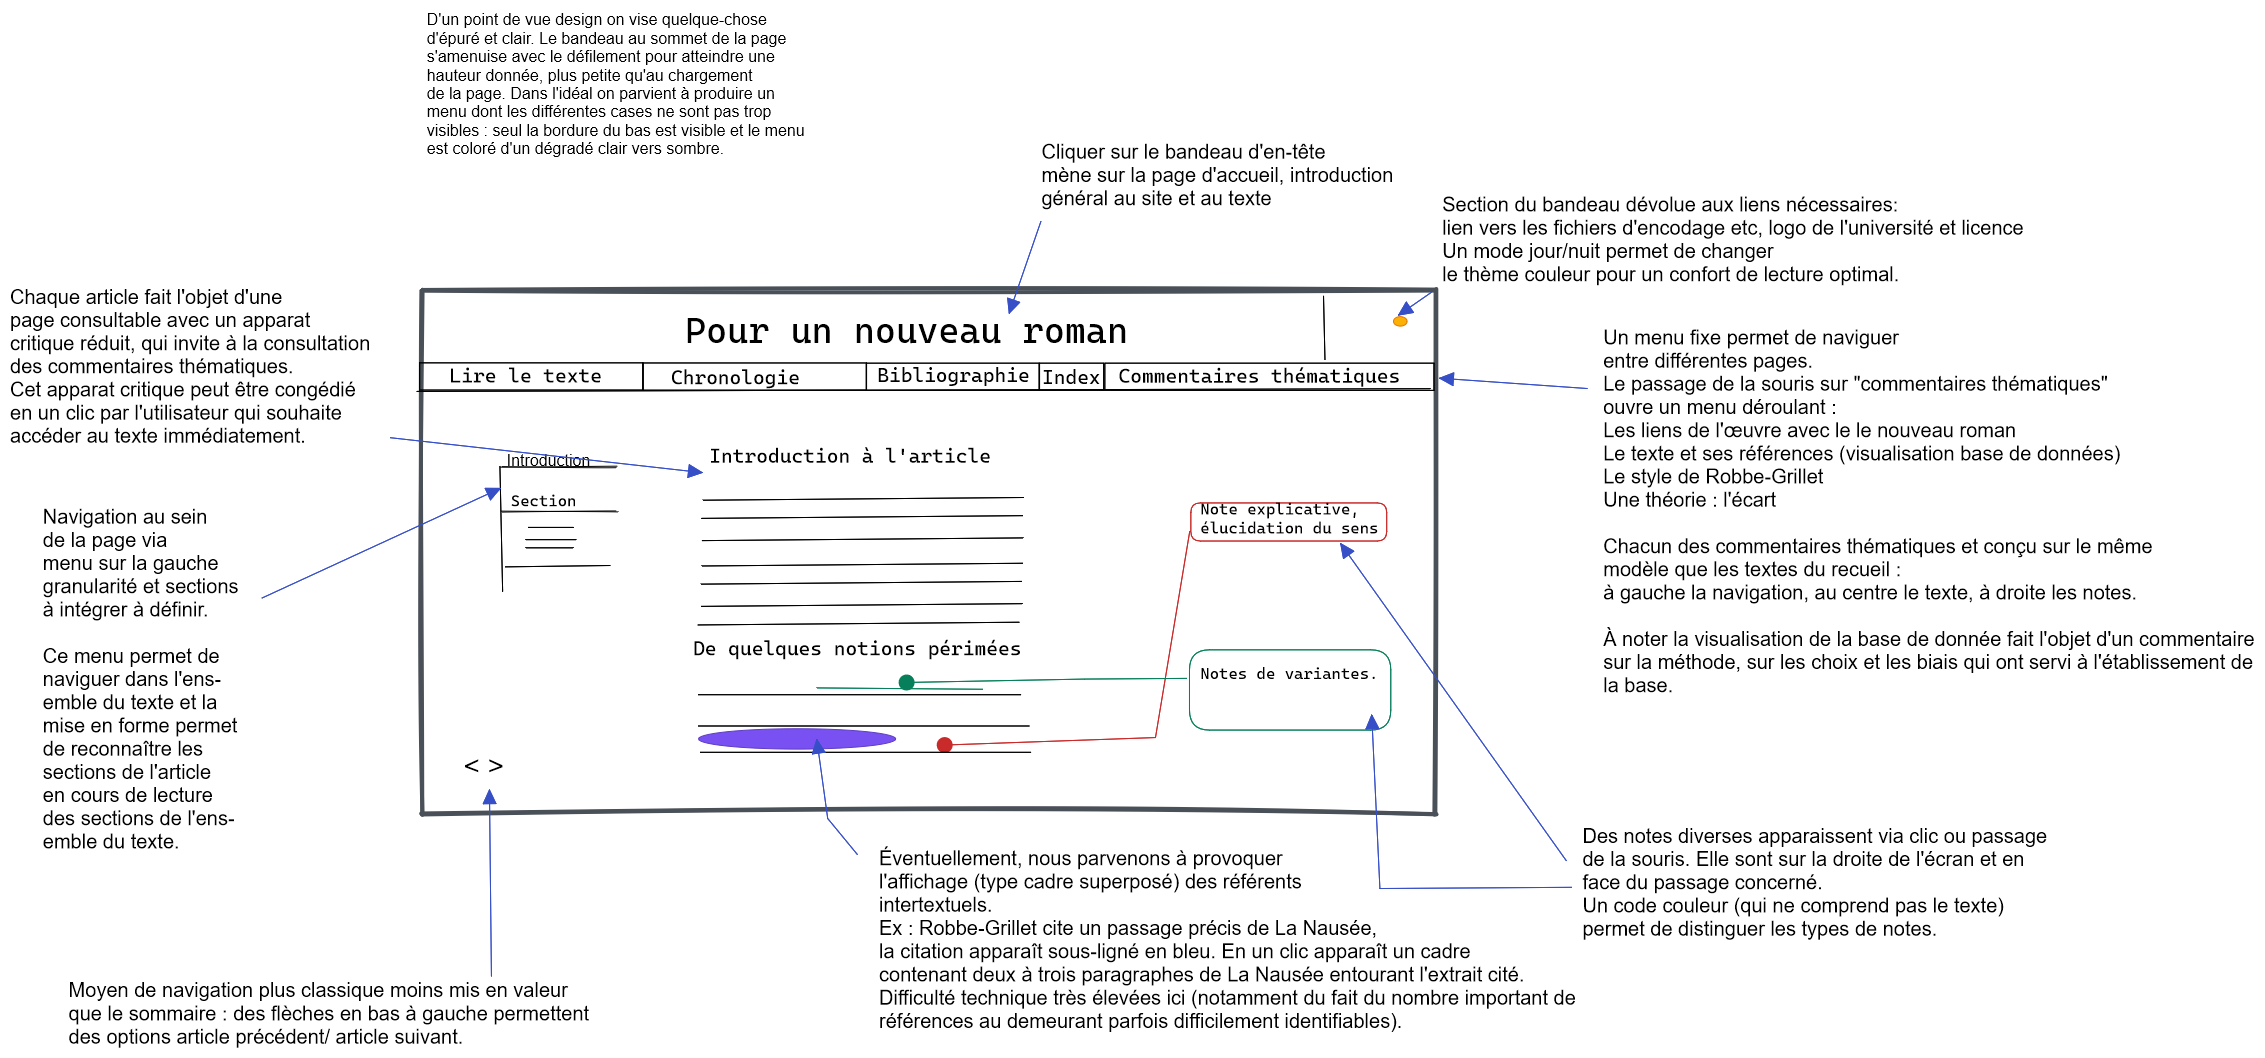
\includegraphics[scale=0.3]{img/202211_mevel_punr_edition_numerique.png}
    \caption{Schéma du projet original}
    \label{fig:projet}
\end{figure}



Nous opérons une première distinction entre «~références~» et «~citations~». Lorsque p.~136 Robbe-Grillet écrit «~\textit{Mahu ou le Matériau}, ce titre est déjà un programme~», il s'agit d'une référence~; mais lorsque au paragraphe précédent Robbe-Grillet écrit «~"J'y pense, j'y pense [...]"~», il s'agit d'une citation.

Un simple clic sur une citation (soit un passage extrait hors du texte de Robbe-Grillet) devait permettre de lire la citation en contexte (soit un ou deux paragraphes entourant le ou les passages cités). La proposition initiale envisageait déjà des limites aux citations à traiter ainsi mais les choix n'étaient pas encore faits. En effet, le nombre de citation à identifier et le temps nécessaire à l'intégration de nombreux extraits relativement conséquents étaient les freins principaux à cette proposition, qui a, depuis été adaptée.


Dans l'état actuel, seules les citations issues des écrits de Sartre font l'objet d'un traitement proprement transtextuel. Nous privilégions cette partie du corpus car nous pensons insister dans le versant scientifique du projet sur les rapports qu'entretient la pensée de Robbe-Grillet dans \punr{} avec celle de Sartre. Ainsi notre édition est-elle la plus proche possible de notre travail scientifique. %lol
Notons que nous ajoutons aux intertextes issus de Sartre, les citations issues des œuvres de Robert~Pinget \textit{Le Renard et la boussole} et \textit{Mahu ou le matériau}. Cet ajout plutôt qu'un autre tient davantage à des raisons techniques que scientifiques~: nous avons mené nos tests de faisabilité technique sur ce corpus.
\begin{itemize}
    \item La diversité de ces œuvres dans lesquelles la digression perpétuelle fait office de narration permettent d'interroger les limites des extraits à intégrer. Afin d'intégrer le contexte d'une citation, il nous fallait déterminer quel était ce contexte~; un ou deux paragraphes~? Une phrase avant et après~? \textit{Quid} alors des cas où les phrases elles-mêmes sont très longues voire déstructurées~? Nous optons pour un découpage dont nous espérons que la cohérence apparaîtra au lecteur~; plutôt que des bornes quantifiables en termes de distance textuelle, nous nous sommes efforcés d'intégrer des extraits tenus par une unité cohérente, que cette unité relève de l'épisode ou de la plus petite digression possible (dans le cas de Pinget).
    \item D'un point de vue technique, les citations issues des œuvres de Pinget nous permettent également d'identifier des citations pouvant renvoyer à plusieurs extraits d'une même œuvre, ce qui nous posait un problème technique que nous avons souhaité résoudre (voir~: \ref{quote_dis}).
    \item Enfin Pinget nous a semblé être l'auteur pour lequel Robbe-Grillet réservait le plus d'éloge. La section «~Un roman qui s'invente lui-même~» est située en fin de l'«~Anthologie~» laissant entendre qu'il s'agit de l'auteur le plus «~moderne~».
    %selon Robbe-Grillet qui écrivait encore dans les années 1990 dans le quotidien \textit{Le Monde} que «~\footnoteB{%REFENRECE }~» %REFERENCE MANQUANTe
    Nous avions ainsi deux des pôles axiologiques mentionnés explicitement les plus éloignés.
    \item La version actuelle (juin 2023) ne contient pour l'instant que les citations de Robert Pinget afin de démontrer, d'une part la possibilité mais aussi l'intérêt d'un tel traitement.
\end{itemize}

Si l'objectif initial, et surtout, idéal, de ce travail était de traiter l'intégralité des citations, le temps nécessaire à un tel travail nous imposa de réduire la voilure.
Ainsi, si toutes les références et citations feront l'objet d'un traitement minime~: en html et css (voir \ref{htmlCss}), nous programmons l'affichage d'une infobulle pour chacun de ces éléments lorsque la souris de l'utilisateur passe dessus, affichant~: les statuts référentiels et axiologiques de la référence ou citation sur laquelle passe le curseur. Un code couleur permet au demeurant d'expliciter les valeurs (rouge, vert, bleu et noir pour les statuts axiologiques et des nuances allant du jaune au maron pour le statut référentiel).

% Dans la version actuelle, le code permettant cet affichage est déjà implémenté et les valeurs déterminées (notamment dans la base de données voir~: \ref{ref:dbEtabValeurs}) mais l'encodage des attributs n'est pas encore terminé (voir \ref{tei}), dès lors l'affichage est encore défectueux sur nombre de ces éléments. Par ailleurs, si la version actuelle met en valeur les références et les citations en leur donnant une couleur particulière (vert et bleu respectivement), la version finale du présent travail se passera de cette mise en forme qui nous paraît nuire au confort de lecture.

Enfin, toujours dans un souci d'offrir la lecture la plus agréable possible, nous choisissons de ne pas produire de note explicative sur la plupart des références.
\begin{itemize}
    \item Le contenu de ces notes nous paraîssait devoir être à la fois trop général et trop court pour avoir un quelconque intérêt scientifique.
    \item Malgré le temps conséquent consacré à concevoir et implémenter ces notes au contenu factuel, l'intérêt pour un lecteur néophyte qui a à sa disposition des encyclopédies en ligne nous paraissait très faible~; plus encore pour un lecteur spécialiste qui n'apprendrait sans doute rien, ou si peu de telles notes.
    \item Ces notes surchargeraient l'appareil critique de notre édition et, au fond, contreviendraient en partie au principe de l'édition~: donner à lire, sans prendre par la main le lecteur, supposé capable de naviguer lui-même au sein de l'édition.
\end{itemize}





Nous nous proposions de fournir pour les articles une table des matières qui permettrait de «~piocher~» dans le recueil des passages de la pensée de Robbe-Grillet. Ces renvois ne sont pas encore implémentés mais le seront prochainement (voir~: \ref{encMilestone}).


\section{Encodage}
Afin de proposer une édition numérique enrichie de \punr, nous optons pour un encodage en XML-tei. Pensé courant octobre et novembre, l'encodage à proprement parler a commencé début mars.
    \subsection{Principes généraux}
Le langage XML est un langage de balisage~: l'encodeur entoure chacun des éléments qu'il juge devoir être encodé (l'ensemble du texte, un paragraphe, un mot, voire une lettre) de balises ouvrantes et fermantes éclairant la nature du passage qu'elles entourent (libre à l'encodeur d'encadrer un paragraphe en tant que paragraphe ou en tant que saut sémantique).

\begin{figure}[H]
    \centering
    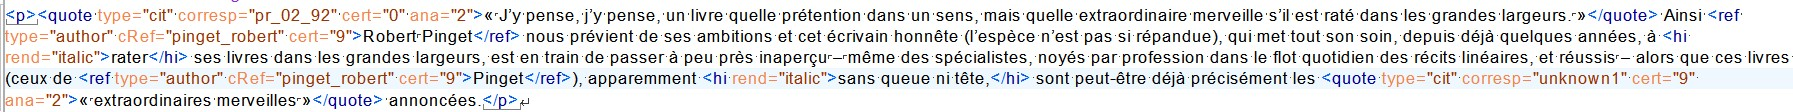
\includegraphics[scale=0.5]{img/screen_encodage.jpg}
    \caption{Exemple d'encodage xml-tei}
    \label{fig:screen_encodage}
\end{figure}

L'encodeur étant libre de choisir les éléments qu'il encode et comment il les encode, des conventions internationales ont émérgé afin de permettre l'interopérabilité des corpus balisés. Le plus utilisé en science humaine demeure sans doute le standard de la \textit{Text Encoding Initiative} (TEI) que nous employons pour la présente édition. Initialement pensé pour la restitution de sources anciennes (tels des manuscrits du \textsc{XVI}\textsuperscript{e}) cet encodage nous permet d'identifier des éléments structurels très fins et de mettre en correspondance différents extraits constituant un corpus (voir \ref{tei}).

Lors du rapport d'étape soumis courant décembre~2022, nous avions l'intention de produire une ODD. C'est-à-dire un fichier permettant la génération d'un schéma et d'une documentation technique sur les choix d'encodage fait pour le présent travail (soit une spécialisation des éléments xml-TEI). Le temps nous a finalement manqué pour produire un tel travail qui nous a paru au demeurant en partie redondant avec le présent document.


    \subsection{Mise en œuvre}


\subsubsection{Un premier fichier d'encodage}
\label{premier_enc}
Afin de pouvoir encoder le texte du \punr{} nous nous sommes procuré une version numérique du texte en achetant la seule édition disponible de l'œuvre au format \go.epub\gf. Nous savons que les fichiers d'un epub se présentent sous la forme d'une archive~: il suffit de changer l'extension «~.epub~» en «~.zip~» pour pouvoir explorer son contenu et en extraire les fichiers contenant le texte.

Ces fichiers se présentent sous la forme de fichiers «~.html~», un fichier par chapitre du recueil. Grâce à un script perl nous récupérons l'ensemble du contenu textuel au sein d'un seul fichier .xml.

Le même script procède simultanément au nettoyage des fichiers d'origine (nous remplaçons les balises html par des balises xml-tei lorsque cela est pertinent et supprimons toutes les balises inutiles).

Ont été supprimés~:
\begin{itemize}
    \item les éléments <div> vides servant à espacer le corps du texte (une indication des suppressions et des tailles des éléments supprimés est à chaque fois ajoutée en commentaire dans le fichier d'encodage)
    \item les éléments <span> parasites qui redoublaient, entre autres, tous les éléments <p> sans ajouter d'information de mise en forme
    \item les éléments <b> et <a> muni d'un attribut @id marquant le début des chapitres
\end{itemize}

Ont été remplacés par les balises xml-tei jugées pertinentes~:
\begin{itemize}
    \item les éléments <a> munis d'un attribut @id signalant les débuts de page par des éléments <pb> munis d'un attribut @n
    \item les éléments <i>, au demeurant dépréciés selon les normes actuelles du web, par des éléments <hi> munis d'un attribut @rend avec pour valeur "italic"
    \item les éléments <p> marquant les paragraphes ont été conservés mais sans leur attribut @class de valeur "txt"
    \item les éléments <h1> marquant les titres ont été remplacés par des éléments <head>
    \item les éléments <h2> marquant les titres de sous-sections (par exemple «~L'intrigue~», sous-section de «~De quelques notions périmées~») par des éléments <head> avec un attribut @type ayant pour valeur "subsection\_head"
    \item les éléments <small> par des éléments <hi> munis d'un attribut @rend avec pour valeur "small-caps"
    \item les éléments <sup> par des éléments <hi> munis d'un attribut @rend avec pour valeur "exposant"
    \item les éléments <blockquote> par des éléments <cit>
    \item les éléments <p> et leurs attributs marquant la mise en forme du nom de l'auteur de la citation mise en exergue, par un élément <ref>
\end{itemize}

Notons que le nettoyage a été effectué en conservant, grâce à des commentaires, les traces de balises supprimées que l'on pourrait vouloir restaurer (tels les éléments <div> utilisés dans les fichiers html d'origine pour insérer du blanc dans le corps du texte).

Nous ajoutons des balises ouvrantes <quote> à chaque fois que le script de nettoyage rencontre le caractère "«" et fermante après le caractère "»", afin d'effectuer un premier repérage automatique des citations ou emprunts, qui seront ensuite complétés et corrigés à la main si besoin. Notons que le script de nettoyage ajoute également ces éléments en début et en fin de paragraphe du segment «~Joë Bousquet le rêveur~» où cela est nécessaire (lorsque \robbe{} cite plus d'un paragraphe il n'insère pas de guillemets, rendant le balisage automatique plus laborieux).

Nous ajoutons également des éléments <div> marquant les sections du texte autour de chaque article du recueil ainsi qu'autour des passages identifiables à des sous-sections (telles les «~notions périmées~») cette fois munis d'attributs @type ayant pour valeur "subsection".

Nous obtenons alors un fichier \go.xml\gf valide qui n'est encore qu'une première étape pour l'encodage complet.

\subsubsection{Vers un encodage XML-TEI en vue d'une édition numérique}
\label{tei}

Afin d'intégrer les références transtextuelles de \punr{} à notre édition pour permettre l'édition enrichie que nous nous proposons de réaliser nous employons un encodage de type «~corpus\gf. 
\begin{figure}[H]
    \centering
    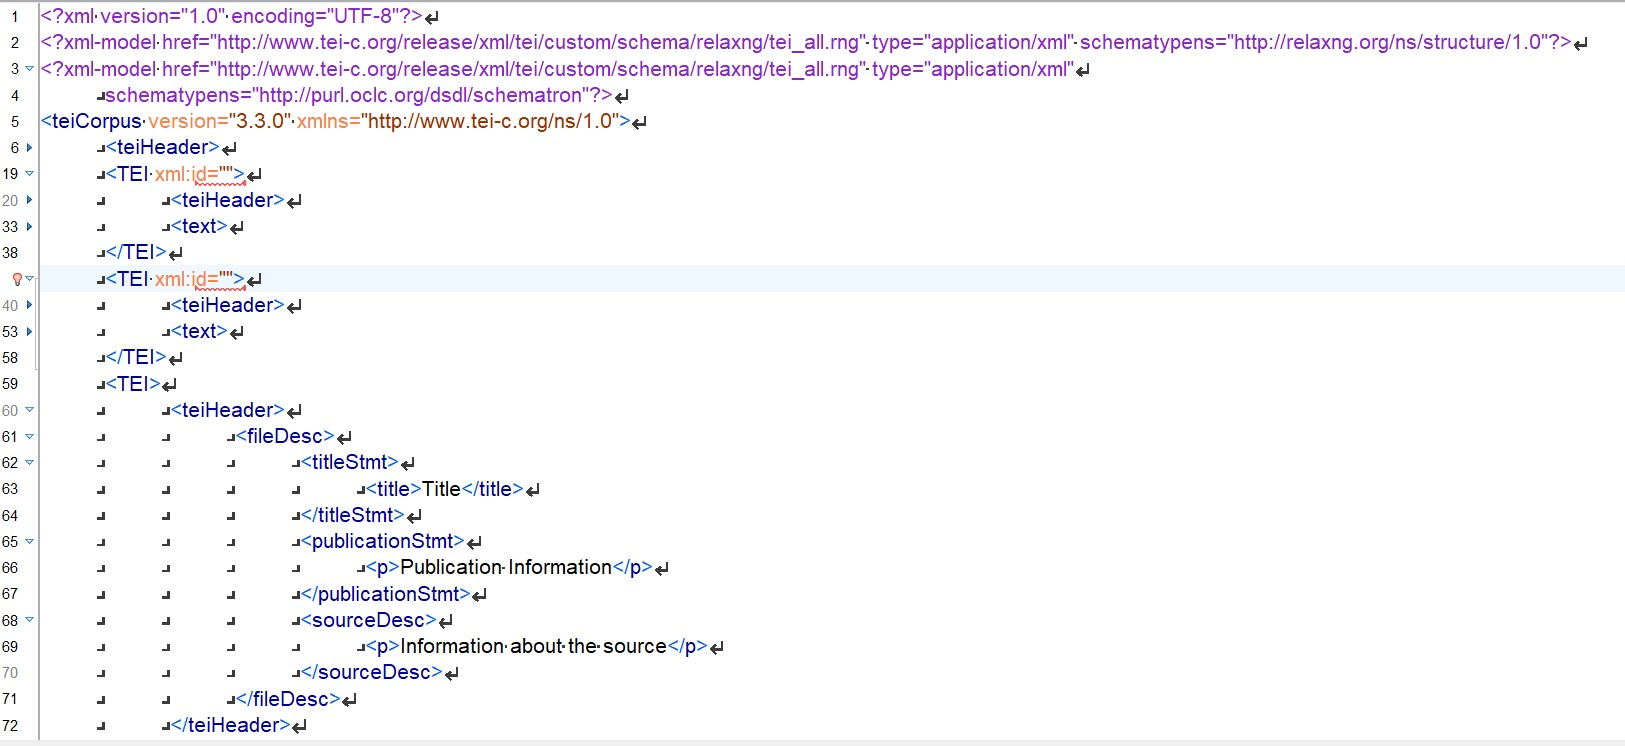
\includegraphics[scale=0.5]{img/screen_itei_corpus.jpg}
    \caption{La structure du fichier d'encoage}
    \label{fig:screen_tei_corpus}
\end{figure}
Alors que la majorité des encodages TEI se contente d'un seul élément <TEI> contenant l'œuvre ou le manuscrit encodé nous employons un élément <corpus> qui contiendra plusieurs éléments <TEI> identifiés grâce à des attributs @xml\NoAutoSpaceBeforeFDP:id. Une version vide du fichier xml a pour cela été produite. Cet xml vide converti au format texte brut est ensuite injecté par le script de fusion et de nettoyage des fichiers qui compose \punr. Il contient~:
\begin{itemize}
    \item un élément <teiHeader> (sorte de carte d'identité du document ou du texte) pour l'ensemble du fichier, contenant des informations succintes sur le projet d'édition auquel est rattaché le fichier.
    \item et quelques éléments <TEI> accompagnés de <teiHeader>, vides pour les extraits des références transtextuelles.
    \item un élément <TEI> et <teiHeader> contenant les informations relatives à l'édition de \punr. C'est cet élément <TEI> dans lequel sera injecté le texte nettoyé et pré-encodé par le script.
\end{itemize}

Si nous reproduisons l'intégralité de \punr{} dans l'élément <text> qui lui correspond nous n'insérons dans les autres éléments <text> que les extraits qui nous intéressent~: nous produisons bien une édition de \punr{} inscrit dans un corpus plus vaste, pas l'édition d'un corpus dont \punr{} ne serait qu'un élément. Extraits transtextuels et passages de \punr{} correspondant sont ensuite liés via un jeu d'attributs @corresp et @xml\NoAutoSpaceBeforeFDP:id.
\begin{figure}[H]
    \centering
    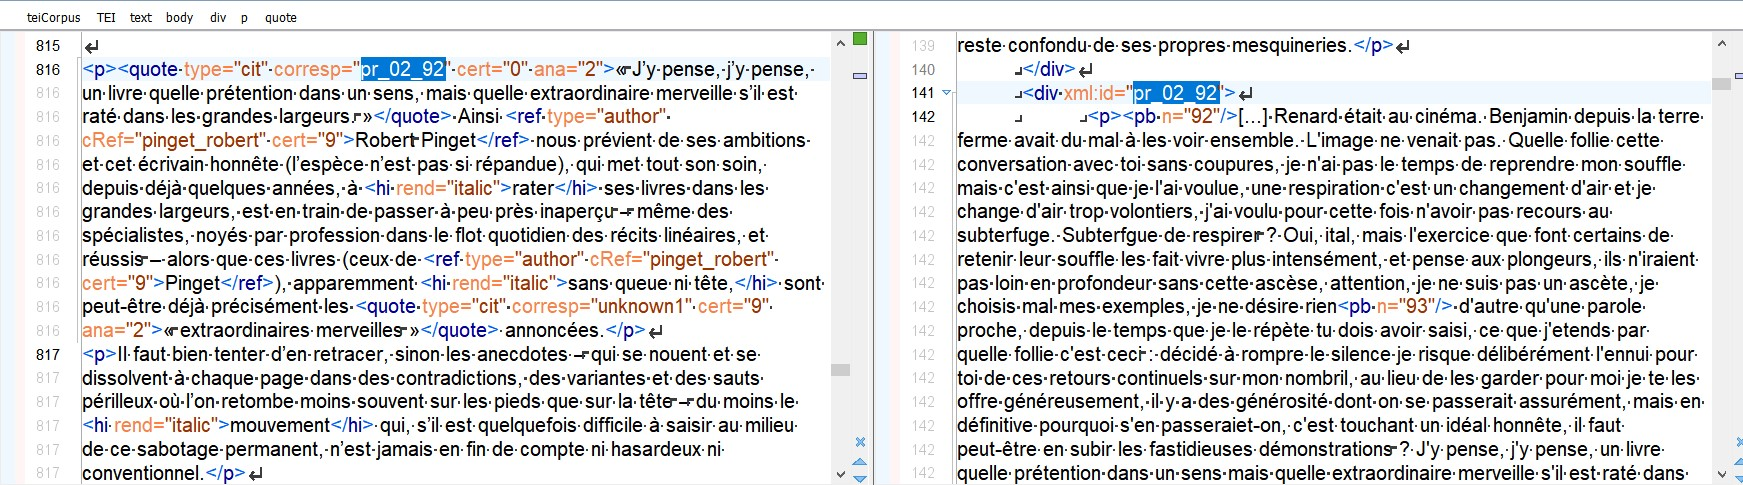
\includegraphics[scale=0.5]{img/screen_corresp.jpg}
    \caption{Exemple de correspondance}
    \label{fig:screen_corresp}
\end{figure}
\subsubsection{Encodage sémantique automatisé}

On désigne généralement par «~encodage sémantique~» l'ajout d'éléments xml identifiant des noms de personnages, des toponymes, des dates, des références, etc. Afin d'accélerer cette étape fastidieuse nous optons pour un premier encodage automatisé. Pour cela, nous ajoutons à notre script de nettoyage des lignes servant à repérer les noms d'auteurs et à les baliser selon le modèle suivant~:
\begin{itemize}
    \item un élément <ref> (référence)
    \item muni d'un attribut @type avec pour valeur "author"
    \item et d'un attribut @cRef (référence canonique) dont la valeur est constituée sur le modèle «~nom\_prenom~». Générée automatiquement par le script, cette valeur comprendra des majuscules et/ou des lettres accentuées (puisque \robbe{} écrit «~Samuel Beckett~» la valeur sera "Beckett\_Samuel"), elle fera l'objet d'une correction grâce à l'emploi d'une feuille xsl.
\end{itemize}
Afin d'éviter le double balisage, nous balisons la dénomination complète («~Samuel Beckett~») en ajoutant un espace insécable entre le prénom et le nom, avant de baliser «~Beckett~» seul, s'il est précédé d'un espace sécable.
% Voir ci-dessous si maintenu~:
%Nous ajoutons ensuite au script de nettoyage les noms des personnages des pièces de Beckett abondamment cité dans l'article «~Samuel Beckett, ou la présence sur la scène~» balisé en tant que <quote> et le concept de «~Nature~» balisé en tant que <ref> avec pour valeur de l'attribut @type "concept" et @cRef "philo\_nature", ainsi que l'Académie française mentionnée deux fois et balisée en tant que <ref> de @type "entité collective". Notons que ces ajouts ont été effectué après l'emploi d'un autre script qui parcourt le texte complet et renvoit tous les mots commençant par une majuscule à l'exception d'une (longue) liste de terme à exclure (tel «~Je~» ou «~ainsi~» commençant une phrase) présent dans le corpus, permettant d'identifier les anthroponymes présents dans le recueil.


Puis grâce à une transformation xsl (voir \ref{ref:xsl_gen})sommaire, nous générons l'affichage des éléments <quote>, <ref> et <hi> munis d'un attribut @rend="italic" afin de les identifier, corriger et compléter si besoin. Cette vérification se fait livre en main~: la transformation renvoie également pour chaque élément identifié à la page à laquelle il apparaît. Cette étape est répétée plusieurs fois, ce qui nous permet de raffiner le balisage automatique à chaque passage.

Avant de passer à l'encodage manuel nous utilisons une autre transformation xsl afin de faciliter cette étape fastidieuse~:
\begin{itemize}
    \item Nous ajoutons des attributs aux éléments <quote> qui n'en ont pas, leurs valeurs doivent correspondre autant que possible aux éléments répertoriés dans notre base de données (voir \ref{ref:db_modele_relationnel}).
    \begin{itemize}
        \item @type correspondant à ttNature
        \item @corresp qui correspond à l'@xml\NoAutoSpaceBeforeFDP:id des extraits cités (encodé en <text>) et aux valeurs de ttIdent définies dans la base de données préfixé de "tt"
        \item @cert qui correspond à mReferenceStatu, soit le statut de la référence (est-elle mentionnée, citée, etc.)
        \item @ana correspondant au mAxiologicStatus (s'agit-il d'un blâme, d'un éloge, ou d'une mention indiférente~?).
    \end{itemize}
    \item Nous modifions les valeurs des @xml\NoAutoSpaceBeforeFDP:id des éléments <div> qui entourent chacun des articles du texte, afin de les faire correspondre aux valeurs de notre base de donnée.
        \begin{itemize}
            \item Par exemple, le chapitre «~À quoi servent les théories~» encodé par un <div> n'aura plus comme valeur de l'@xml\NoAutoSpaceBeforeFDP:id "page006" mais "1". L'utilisation des pages comme identifiants nous paraît superflue, vu la présence d'éléments <pb> à chaque début de page.
        \end{itemize}
    \item Nous retouchons les titres (de sections et de sous-sections) afin de corriger l'encodage d'origine qui encodait chacune des lignes d'un titre ou sous-titre ainsi que les dates dans deux éléments <head> différents. Les capitales sont également remplacées par des minuscules qui seront plus tard affichées en petites capitales.
    \item Les mentions des dates sont intégrées aux titres et encodées en tant que <date> avec un attribut @rend dont la valeur est "italic". Par ailleurs, nous en retirons les parenthèses qui provoquaient une erreur sans doute due au moteur d'expression régulière d'Oxygen\footnoteB{En expression régulière, les signes «~()~» servent à garder en mémoire les caractères qu'ils contiennent. Or, notre transformation recourait au moteur d'expression régulière inclus dans Oxygen pour intégrer les dates au titre. Ceci provoquait une erreur~: la transformation considérait que les caractères «~()~» devait être interprétés comme des délimiteurs d'expression régulière et non comme le contenu à supprimer, ainsi les dates étaient bien supprimées mais pas les parenthèses les entourants.}, les parenthèses seront rétablies dans la version html de l'édition.
    \item Tous les autres éléments et attributs déjà présents sont reproduits à l'identique. Par là nous nous assurons de pouvoir réappliquer la transformation sur notre fichier d'encodage manuel autant de fois que nécessaire. Nous nous contenterons de modifier le nom du fichier de sortie afin de ne pas écraser les précédentes itérations. Ainsi nous pouvons appliquer des corrections «~en cours de route~» sans perdre les ajouts manuels.
\end{itemize}


\subsubsection{Encodage sémantique à la main}
Certains contenus textuels ne peuvent être repérés automatiquement et nécessitent donc d'être encodés à la main.

En effet il convient d'attribuer les bonnes valeurs aux attributs, voire de rectifier l'encodage automatique qui ne peut, par exemple, distinguer entre la mention à la page~164 d'un titre «~L'Année dernière à Marienbad~» et la mention d'un élément diégétique de cette œuvre «~se sont-ils vraiment rencontrés, aimés, l’année dernière à Marienbad~?~» un peu plus loin.

Notons par ailleurs les difficultés à limiter le balisage. En effet l'on pourrait considérer certains éléments diégétiques, tels les allusions aux personnages des œuvres de Beckett ou les supposées réactions sus-citées que \robbe{} prête au public comme devant être encodées en tant que <quote>~: citer un personnage d'une œuvre, n'est-ce pas citer l'œuvre~? ces réactions mêmes (re)constituées par \robbe{} ne sont-elles pas des éléments textuels mobilisés par \robbe{} à la manière de citation à réfuter~?

Pour régler ces difficultés nous nous appuyons sur les objectifs que nous nous sommes fixés au moment où nous avons élaboré ce projet d'édition numérique~: nous souhaitons produire une édition qui expose les relations transtextuelles de \punr{} pour le replacer dans son époque, ou plutôt pour donner les représentations que le texte produit de son époque. Dès lors, il nous paraît opportun de baliser les réactions du public décrites ou (re)constituées par \robbe{} afin de permettre de les comparer à la réalité de ces réactions. Au contraire les paraphrases (surtout si elles sont exactes) d'œuvres longuement commentées par \robbe, ne nous intéresse que modéremment. La source identifiée, ou plutôt, vérifiée, l'intérêt des passages cités n'ont que peu d'interêt par rapport au commentaire dans son ensemble.

De manière plus anecdotique, la recherche de chaînes de caractères contenant des apostrophes telles «~L'Étranger, L'Immortelle~» pose un problème épineux à résoudre car l'apostrophe est le signe utilisé par le moteur de recherche pour délimiter la chaîne. On écrit 
\begin{itemize}
    \item 'L'étranger', 
    \item 'L\&apos;étranger',
    \item 'L''''étranger'~; 
\end{itemize}
le moteur renvoie une erreur. Après quelques essais nous abandonnons la correction de ce segment~: pour moins d'une dizaine de mentions aisément identifiées à la main, chercher une solution trop longtemps ne présentait aucun intérêt.
% blabla


L'encodage des sources citées se fait également à la main, chacun des textes du corpus est ajouté aux éléments <TEI> munis d'un attribut @xml\NoAutoSpaceBeforeFDP:id servant à l'identifier sur le modèle~: initialdel'auteur\_numérodel'œuvre~» ainsi \textit{Mahu ou le matériau} sera désigné par «~pr\_01~» et \textit{Le Renard et la boussole} par «~pr\_02~». Chacun des extraits est ensuite inséré dans un élément <div> ayant aussi un attribut @xml\NoAutoSpaceBeforeFDP:id construit sur le modèle~: iddel'œuvre\_pagededébutdelacitation~», ainsi le premier extrait de \textit{Le Renard et la boussole} correspondra à «~pr\_02\_09~».    

\label{encMilestone} Nous employons des éléments <milestone/>, bornes, pour inscrire les points rhétoriques importants. Lors de la transformation XSL ces <milestone> seront transformés en élément <a/>, \textit{anchor} ancre, ces éléments sans contenu seront invisibles au lecteur mais permettront de constituer un menu de navigation sur la gauche de l'écran en XSL (voir \ref{ref:xsl-gen}). Leur attribut @id construit sur le modèle~: «~refutation2~»
sera d'une part nécessaire à la bonne exécution du script (le lien hypertexte créé dans la navigation renvera vers cet identifiant unique à chaque ancre au sein du texte) et permettra de produire un nom compréhensible dans le menu~; «~refutation2~» sera analysé par la transformation qui écrira dans le lien hypertexte «~Deuxième réfutation~».



Les index des concepts adverses et des expressions privilégiées constituent des outils à l'usage des chercheurs mais également un point d'entré ludique dans le corpus.

 \label{encW} Les expressions devant figurer dans ces index sont encodées en tant que <term/>, «~terme (considéré technique)~»au sein d'éléments <span> «~passage lié à une interprétation~», munis d'attributs @type dont les valeurs «~0~» ou «~1~» orientent grâce à la transformation XSL, le mot vers l'index des concepts adverses ou des expressions privilégiées, respectivement. Les éléments <span> englobe l"expression et son contexte permettant de l'expliciter (en effet la recension des adjectifs «~vrai~» ou «~difficile~»  seuls serait de peu d'intérêt), l'expression encodée en <term> est ensuite mise en valeur via css, en rouge ou vert pour les notions adverses ou les expressions privilégiées respectivement.

Dans une version précédente soumise à évaluation nous nous proposions d'encoder ces éléments avec le couple <w/> «~\textit{word}~» et <ab/> «~\textit{arbitrary segment}~». Cette solution a finalement était rejetée car elle n'était pas valide en xml-tei. Aussi, nous sommes-nous orientés vers des éléments plus spécifiques~: employant des chercher/remplacer pour remplacer tous les élémnents <w/> déjà placés en élément <term/>.<br />Enfin, notre transformation xsl de balisage semi-automatique, légèrement modifiée nous permit de faire remonter l'attribut @type placé sur les éléments <w> sur les éléments <span>.


Ces deux index prennent la forme de deux pages du site que le lecteur trouve dans un menu déroulant de la navigation en haut de page «~Commentaires thématiques~». Après une courte introduction chacun des termes utilisés est listé avec une mention de page et en un clic sur le numéro de page, le lecteur peut être redirigé vers le passage du texte concerné. Si aucun des termes ne fait l'objet d'un commentaire spécifique (autre qu'à titre d'exemple), une introduction générale aux index est intégrée. Cette introduction sert à présenter cette part du travail et également à délivrer un commentaire sur l'aspect stylistique ici mis en valeur. Il ne nous a pas semblé opportun d'ajouter un commentaire pour chaque terme, d'une part car ces termes sont rarement en eux-mêmes des termes difficiles («~personnage~», «~intrigue~» etc.) et d'autre part car un renvoi vers le passage du texte où le terme est employé nous semblait un outil bien plus intéressant autant pour le lecteur expert que pour le lecteur néophyte. Enfin, il nous semble que c'est en tant que système que ces expressions font sens. 


% pour partie scientifique
% pour partie scientifique
% pour partie scientifique
% pour partie scientifique
Les choix d'encodages des <term/> méritent commentaire. En effet, si l'intuition d'origine avait pour origine les mises en valeurs typographiques de certains termes, mis entre guillemets sans être des citations ou mis en italique, il semblait évident que tous les termes entre guillemets ne méritaient pas d'être intégrés en tant que «~notions adverses~» et tous les termes en italiques en «~expressions privilégiées~»~; certains étaient des citations d'autre un simple procédé d'emphase. Or, à bien y regarder les termes encodés en expressions privilégiées n'étaient pas tous des effets d'emphase~? Ne voit-on pas plutôt Robbe-Grillet insister sur telle ou telle formulation par opposition à une autre explicitement mentionée ou non~? C'est en tout cas ce qui nous est apparu après un examen minutieux. En effet, les expressions privilégiées loin de revêtir l'évidence de concept nettement défini sont davantage des adjectifs qui changent le sens des termes qui les entourent et font signe vers les concepts d'une philosophie, du moins d'une esthétique qui se définit surtout par son opposition à la métaphysique éculée contre laquelle Robbe-Grillet engage son texte. Ainsi les articles indéfinis «~\textit{des} questions, et \textit{des} réponses~» page~64, l'adjectif «~vrai~» pages~24 et~162 (3~fois) et les multiples occurences du verbes «~être~» souvent accompagné de l'adverbe «~là~» (pages~20, 21, 177), expressions privilégiées contenant une assertion possitive sont-ils parmi les termes les plus courants de la langue française et, seul, difficilement rattachable à telle ou telle théorie ésthétique, si ce n'est à une insistance sur l'immanence opposée à la métaphysique prêté aux adversaire de \robbe{}. Sans doute la relative banalité des termes mis en avant par la typographie sert à la démonstration~: l'acceptation de l'immanence des choses difficilement contestable se trouve aussi dans ce choix typographique qui sert à démontrer avec force que l'évidence, c'est-à-dire le bon sens est du côté de Robbe-Grillet.



Notons que l'appréciation «~privilégiées~» porte bien sur la formulation et non le contenu sémantique~: «~Aussi le livre n’est-il pas écrit dans un langage [...]. Seuls, en effet, les objets déjà chargés d’un contenu humain flagrant sont neutralisés, avec soin, et \textit{pour des raisons morales}~» page~69, n'est pas privilégié le fait de choisir son style pour des raisons morales mais bien le propos de Robbe-Grillet sur le style de \textit{L'Étranger}, et ce, peu importe le statut axiologique de ce style au sein de \punr{}.
% pour partie scientifique
% pour partie scientifique
% pour partie scientifique
%pour partie scientifique

%ajouter le passage sur les choix car ARG != systématique






\section{Vers l'édition numérique : transformation XSL}
\label{ref:xsl_gen}
Une fois l'encodage terminé, l'encodeur conçoit une transformation XSL, soit un fichier contenant des informations de traitement afin de passer d'un fichier XML peu lisible pour le lecteur à une édition numérique pour une lecture dans un navigateur web. En effet les feuilles de styles XSL permettent de conserver le fichier XML originel pour en créer d'autres de types divers, en l'occurence nous nous contentons de produire un site internet, soit des pages au format HTML. Notons que le langage de balisage HTML est un dérivé de l'XML qui ne permet pas de structurer le contenu aussi finement que l'XML mais permet un affichage via navigateur web pour lecture.
    \subsection{Principes généraux}
Les transformations XSL fonctionnent par \textit{template}, patron, qui commande le traitement d'un ou de plusieurs éléments XML selon des restrictions diverses laissées au soin de l'auteur de la transformation. On peut par exemple transformer un élément <quote> muni d'un attribut @corresp en un lien hypertexte, qui, lié à des scripts (voir \ref{js}) permettra l'affichage de contenus supplémentaires. 
    \subsection{Mise en œuvre}

Pour tenter d'éviter une écriture redondante nous nous efforçons de produire des templates efficaces et réemployables. Par exemple pour constituer les pages html de notre édition numérique il nous faut générer autant de «~<header/>~» (soit la section au sommet de la page) qu'il y a de pages. Aussi, nous contentons-nous de n'écrire qu'une seule fois le «~<header/>~» (et tous les éléments identiques sur toutes les pages) au sein d'un template nommé qui est ensuite appelé à chage génération de page avec des paramètres permettant de modifier quelques éléments essentiels qui doivent bien être uniques (tel le titre de la page).
%screen du template head et header
\begin{figure}[H]
    \centering
    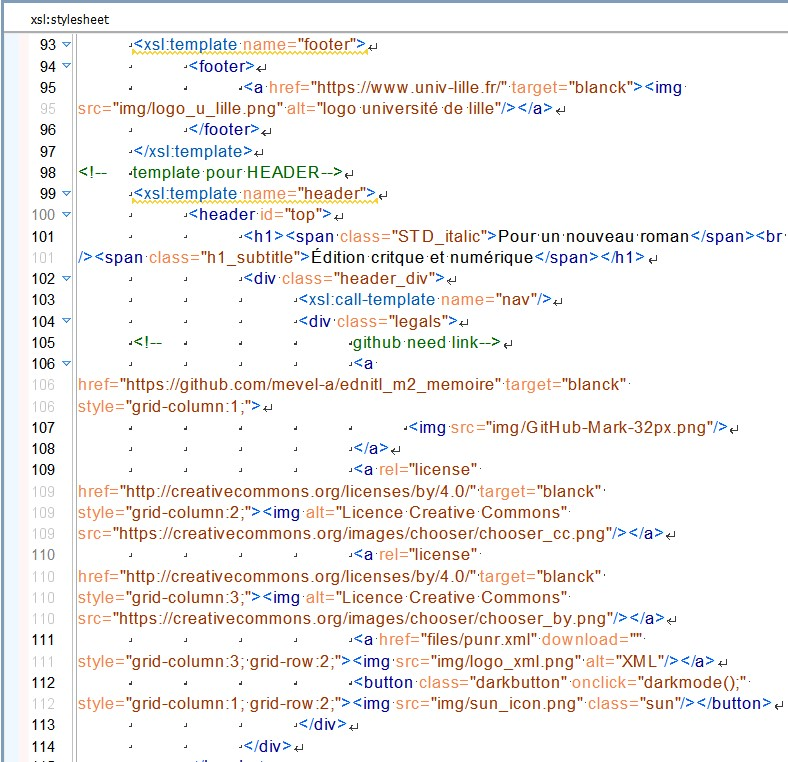
\includegraphics[scale=0.5]{img/screen_header.jpg}
    \caption{Templates gérant le bas (footer) et le haut (header) des pages}
    \label{fig:enter-label}
\end{figure}



Notons que la production des pages est générée par un template matchant la racine du document xml et appelant le template nommé «~body~» qui lui-même appelle les templates \go<header>\gf, \go<footer>\gf, etc. adaptant le contenu de la page selon des paramètres déclarés au moment de l'appel du template.
%screen du template body
\begin{figure}[H]
    \centering
    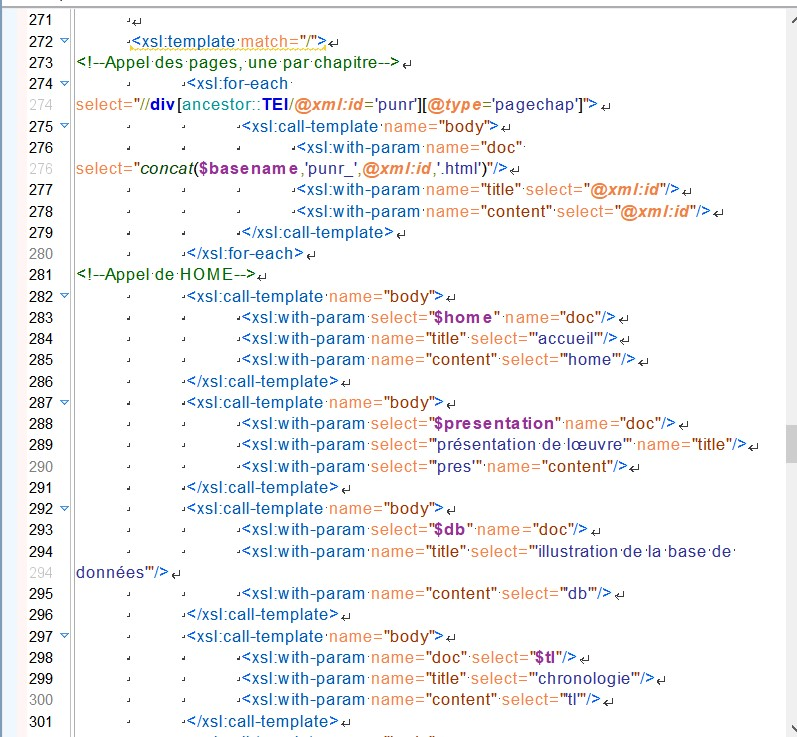
\includegraphics[scale=0.5]{img/screen_body.jpg}
    \caption{Extrait du template gérant la génération des pages du site}
    \label{fig:enter-label}
\end{figure}

\section{Résultat de la transformation : html et css}

\label{htmlCss}

Nos feuilles XSL ont transformé notre document xml difficilement lisible par un lecteur en plusieurs documents html, qui, liés à un fichier css, deviennent bien plus lisibles.

Architecture du web, le langage html est, comme le langage xml dont il est un dérivé, un langage de balisage. Il s'agit ici encore de baliser des segments textuels en vu de les décrire mais contrairment à l'xml les balises utilisables en html sont limitées afin d'être interprétables par un navigateur internet. Parmi ces balises on trouve~:
\begin{itemize}
    \item <p/>, un paragraphe,
    \item <span/> un segment de texte,
    \item <a/> une ancre, ou lien hypertexte.
\end{itemize}
Si le html intervient au niveau sémantique, le css \textit{Cascading Style Sheeet}, lui, sert à la mise en forme. C'est ce langage qui permet de transformer des segmentations sémantiques en véritable boîte sur la page ou de mettre en valeur (par un jeu de couleur par exemple) tel ou tel élément des pages.

\subsection{Les notes de l'édition critique : création d'infobulles}

\label{htmlCssInfo}

%figure{screen_cssinfo.png ou truc du genre}

Les interactions html/css permettent de générer des affichages utiles à notre édition numérique. Détailler avec précision les choix esthétiques et pratiques que nous avons été amené à faire n'aurait sans doute que peu de sens, cependant le travail effectué sur les infobulles mérite d'être examiné en détail, afin d'expliciter la manière dont le css agit sur le html.




Comme en xml-tei, nous disposons d'attributs spécifiques au html pour caractériser nos éléments. Parmi eux l'attribut @class est d'une utilité particulière pour permettre les interactions entre html et d'autres langages de programmation (dans le cas de notre travail css et Javascript). Ces attributs @class et leurs valeurs sont générés par notre transformation xsl et nous avons, dans le cas des infobulles un résultat qui ressemble à ceci~:

\begin{verbatim}
    <span class="ref">contenu sur lequel porte la note<span class="refinfo">la
note elle-même</span></span> la suite du contenu
\end{verbatim}
, soit deux éléments <span/>, segments textuels, le second muni d'une classe «~refinfo~» à l'intérieur du premier classé «~ref~» contient le contenu de la note qui sera en infobulle. L'affichage standard d'un tel code serait le suivant~:
\begin{verbatim}contenu sur lequel porte la notela note elle-même la suite du contenu\end{verbatim}
Or nous souhaitons que le second segment ne s'affiche que lorsque le curseur passe sur la souris. C'est ici qu'intervient le css.

\begin{figure}[H]
    \centering
    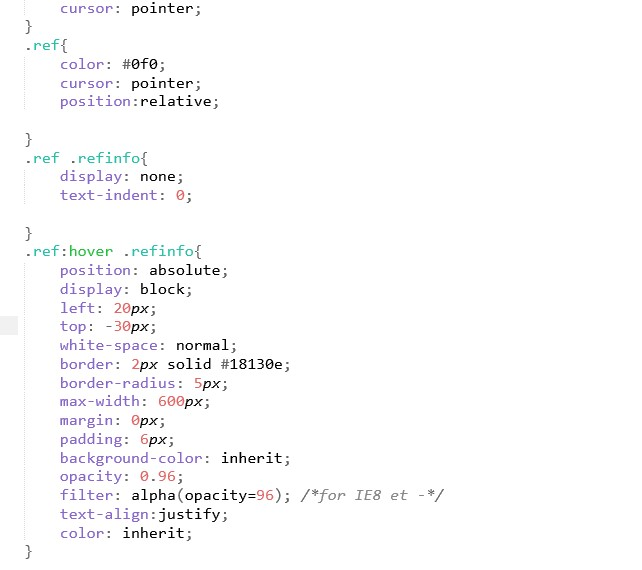
\includegraphics[scale=0.8]{img/screen_css_infobulle.jpg}
    \caption{Le code css gérant les infobulles}
    \label{screenCssInfo}
\end{figure}

\subsubsection{Les notes liées aux références transtextuelles}

Comme on peut le voir dans la figure \ref{screenCssInfo}, css emploie des \textit{selector} auquel il attribue des propriétés. En l'occurence la \textit{class} «~ref~» est sélectionnée ligne~299 et lui est attribuée une couleur (vert) ligne~300.

Nous intéresse davantage le selecteur (ou plutôt les sélecteurs additionnés pour restreindre les éléments ciblés) suivant «~.ref .refinfo~» qui se lit~: l'élément classé «~refinfo~» contenu dans un élément classé «~ref~». Ligne~304 lui est attribuée la propriété «~display:none~» qui empêche l'affichage de l'élément, le contenu de l'infobulle sera présent mais invisible. Il ne sera rendu visible que grâce à la propriété «~display:block~» attribuée aux éléments concernés par les sélecteurs «~.ref:hover .refinfo~», soit l'élément classé «~refinfo~» contenu dans un élément classé «~ref~» sur lequel l'utilisateur passe la souris (on parle de \textit{pseudoclass} pour désigner le sélecteur «~hover~»). Les autres propriétés correspondent à des choix de designs pensés pour rendre l'infobulle lisible et pratique, ainsi les propriétés de positionnement «~position:absolute;left:20px;top:-30px;~» servent à ordonner le positionnement des infobulles selon une position absolue déterminée par rapport au dernier ancêtre positionné (en l'occurence l'ancêtre classé «~ref~» muni de la propriété «~position:relative;~»), le navigateur soustrait à ce point de référence 30~px depuis son sommet (l'infobulle apparaît plus haut) et y ajoute 20~px depuis la gauche (l'infobulle est légérement décallée à droite).

Un tel résultat pourrait être atteint en Javascript mais l'execution d'un tel script serait légèrement plus lourde pour le navigateur et son écriture plus complexe que quelques propriétés css correctement agencées. Notons que les attributs @class ne sont pas seulement utilisés par le css mais également exploité par les scripts détaillés infra.

\subsubsection{Notes critiques non liées aux références transtextuelles}

Nous pourrions souhaiter ajouter des notes explicatives sur le corpus, ou simplement des notes type notes de bas de page au sein de nos commentaires.

S'il suffit pour les notes de nos commentaires d'être insérées directement au sein de des éléments html approprié pour se comporter comme des infobulles, l'ajout de note au sein du corpu nécessite un encodage particulier. Nous choisissons d'encoder le contenu de la note en tant qu'élément <note/> que nous insérons au sein d'un élément <span/> (sans attribut @type) qui contiendra la portion de texte concernée par l'annotation et l'annotation au sein de l'élément <note/>. Après quoi, notre transformation xsl vers html produit un élément <span/> classé « note » contenant l'élément <span/> classé « noteinfo » contenant le contenu de la note. Ces éléments sont classés différemment des notes liées aux références afin de permettre d'en distinguer la nature, mais leur fonctionnement est strictement identique (elles sont liées aux même propriétés css).





\section{Une expérience de lecture~: ajouts de scripts}
\label{js}
    \subsection{Script pour la lecture}

\subsubsection{Javascript, présentation générale}
Afin de permettre l'interactivité d'une page, nous employons un langage de programmation extrêmement courant~: javascript. Ce langage de programmation permet la programmation de fonctions qui, selon l'élément sur lequel clique l'utilisateur, provoqueront tel ou tel comportement au sein de la page.

Une «~fonction~» est une suite d'instructions parfois conditionnées par des «~paramètres~», des informations extérieures à la fonction qui y sont injectées.

\subsubsection{Afficher les citations}
\label{quote_dis}
% Afin d'expliciter la manière dont nous avons travaillé ces scripts, nous souhaiterions proposer une explication détaillée des techniques permettant l'affichage des extraits cités.

% dans img/screen_quote_Xsl et Js1 et 2

La première fonction que nous développons sert à afficher les extraits des autres œuvres cités ou mentionnés par \robbe. Nous choisissons de programmer un affichage que nous espérons élégant et pratique. En bas à droite de la page apparaît un encart contenant l'extrait cité, sa source et des informations quant à l'emploi de la citation (est-ce une «~mention~», est-ce un «~blâme~» ou un «~éloge~»?). L'encart est censé permettre de continuer à lire \punr{} sans avoir à le refermer. Moins élégant peut-être qu'une version qui obscurcirait le reste de l'écran, nous pensons que permettre tel usage correspond davantage à ce que souhaiterait un lecteur effectif.
\begin{figure}[H]
    \centering
    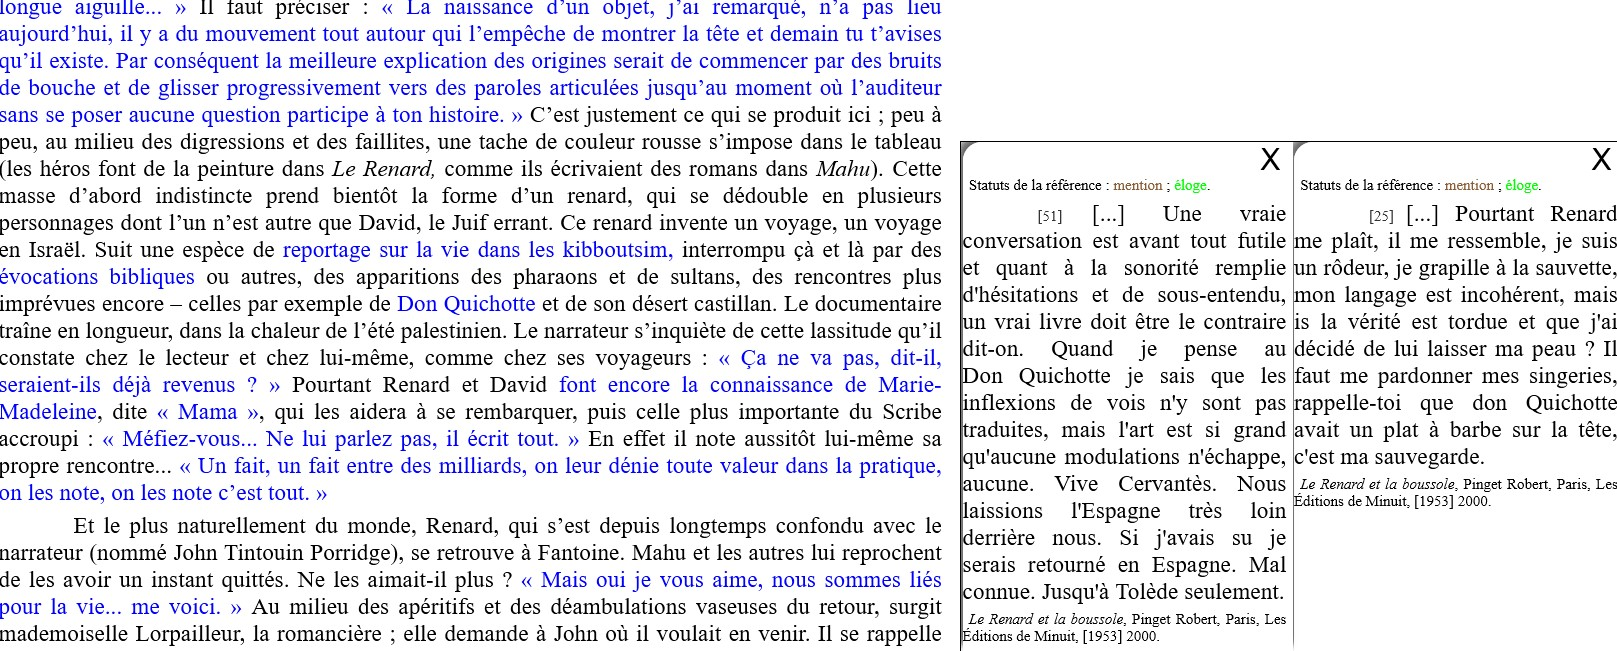
\includegraphics[scale=0.5]{img/screen_quote_result.jpg}
    \caption{Capture d'écran du résultat obtenu}
    \label{fig:quote}
\end{figure}


Au moyen de notre transformation xsl, nous créons pour chacune des citations l'appel d'une fonction qui recevra en paramètre (selon la citation) l'identifiant du passage cité.


On remarque que l'on injecte en paramètre l'identifiant (@corresp) du passage cité, et les statuts référentiels et axiologiques de la référence (@cert et @ana, respectivement) ainsi qu'un dernier paramètre dont les valeurs possibles sont «~1~» ou «~0~» qui sert à orienter le comportement de la fonction nommée «~displayExtract~».

\begin{figure}[H]
    \centering
    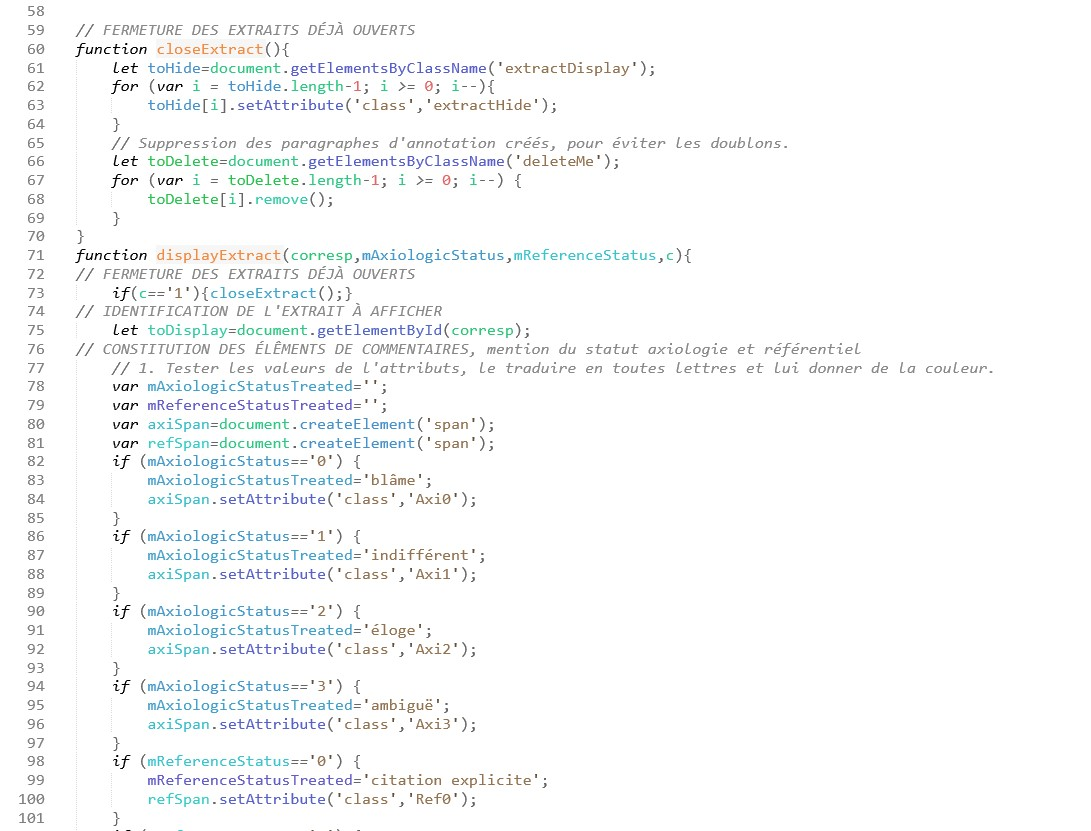
\includegraphics[scale =0.4]{img/screen_quote_js1.jpg}
    \caption{Extrait du script gérant l'affichage des extraits cités}
    \label{fig:displayExtract1}
\end{figure}
\begin{figure}[H]
    \centering
    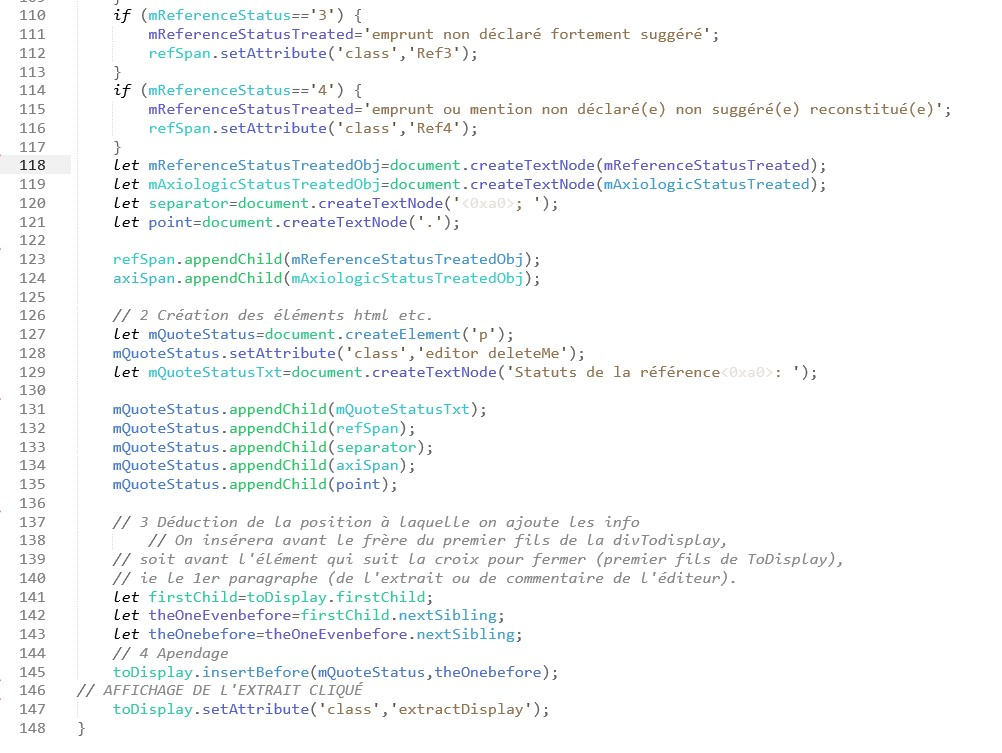
\includegraphics[scale =0.4]{img/screen_quote_js2.jpg}
    \caption{Extrait du script gérant l'affichage des extraits cités}
    \label{fig:displayExtract2}
\end{figure}


En effet, cette fonction n'a qu'à rendre visible le passage concerné lorsque l'utilisateur clic sur une citation. Cependant les choses se compliquent dès lors que nous souhaitons afficher plus d'un extrait pour une même citation. En effet, la même citation par exemple «~Don~Quichotte~» dans l'article «~Un roman qui s'invente lui-même~» peut renvoyer à plusieurs passages de \textit{Le Renard et la boussole}. Or l'encodage xml-tei nous permet précisément d'insérer plusieurs valeurs à l'attribut @corresp séparées par un espace.

On aura donc~: \verb|<quote corresp="pr_02_25 pr_02_50">Don Quichotte</quote>| à prétraiter car notre script Javascript ne peut recevoir qu'une seule valeur en paramètre et ne sera pas capable d'interpréter une suite de valeurs comme telle. Dès lors nous avons opté pour un prétraitement en xsl (voir \ref{fig:corrspAfect}).


Nous souhaitons arriver au résultat suivant~: \begin{verbatim}<span onclick="displayExtract(pr_02_25_02);displayExtract(pr_02_25_50);>Don
Quichotte</span>\end{verbatim}, soit «~lorsque l'utilisateur clique sur ce segment la fonction displayExtract est appelée deux fois sur deux extraits différents. Pour ce faire nous devons séparer les deux valeurs et répéter la valeur de l'attribut @onclick en ne changeant qu'un seul paramètre. Dans un premier template xsl nous testons la présence ou non d'un espace au sein de la valeur @corresp. S'il y a un espace une première partie de la valeur de l'attribut @onclick (soit un premier extrait) est gérée après quoi un autre template est appelé. Ce template nommé «~correspAffect~» reçoit en paramètre tout le contenu de l'attribut qui suit l'espace, il procède ensuite de même~: gère le premier extrait en créant l'appel de la fonction sur ce qui précède l'espace (soit le deuxième extrait), puis via un appel recursif va gérer les unes après les autres toutes les valeurs de l'attribut @corresp après l'espace. S'appelant lui-même le template boucle sur une partie toujours plus réduite de l'attribut @corresp qui correspondra à autant de paramètres ensuite envoyés dans le Javascript jusq'à ce qu'il n'y ait plus d'espace au sein du reste de @corresp, alors, le template produit un dernier appel à la fonction (s'il n'y a plus d'espace il reste l'identifiant d'un extrait) puis s'arrête.

\begin{figure}[H]
    \centering
    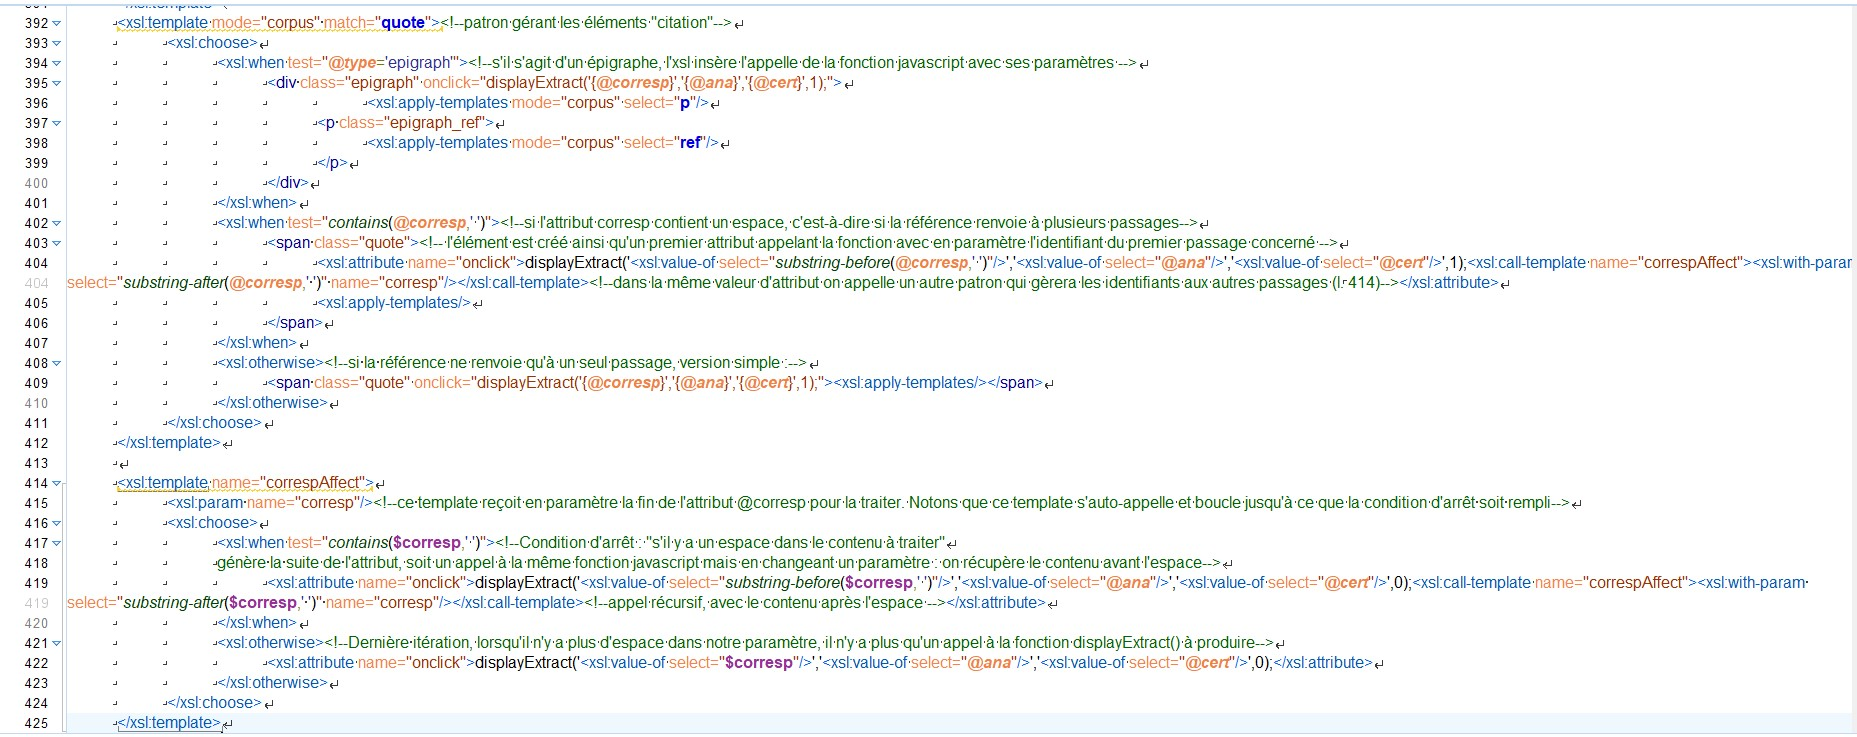
\includegraphics[scale=0.5]{img/screen_quote_xsl.jpg}
    \caption{Le template correspAffect qui sépare les correspondances multiples}
    \label{fig:corrspAfect}
\end{figure}


%back to JS

Une fois tous les appels à la fonction générés, il convient de permettre à la fonction elle-même d'afficher effectivement ces extraits. En effet, afin de permettre au lecteur de refermer un encart contenant un extrait à volonté, nous avons créé une fonction qui repère les extraits affichés (s'il y en a) et les cache (on revient donc à la situation initiale). Cette fonction est attachée à un segment en haut des encarts des extraits où un «~X~» symbolise efficacement une croix.
Cependant il paraît très probable que le lecteur ne ferme pas lui-même les encarts, nous l'encourageons d'ailleurs à le faire en lui permettant de continuer à lire le texte sans (trop) d'encombrement visuel. Aussi avons-nous décidé d'appeler la fonction refermant les encarts ouverts au sein de la fonction les affichants avant qu'elle ne les fasse apparaître.
Lorsqu'un seul extrait est à afficher cela ne pose pas de problème~: la fonction ferme les encarts affichées puis ouvre celui sur lequel le lecteur a clic. Cependant dans les cas où plusieurs extraits sont à afficher, la fonction les affichera puis les cachera de nouveau jusqu'au dernier appelé. Nous ajoutons donc un dernier paramaître à cette fonction~: «~c~» dont les valeurs («~0~» ou «~1~») détermineront si la fonction doit, ou non, cacher les extraits précédemment affichés. 
%capture d'écran fonction JS
Ainsi voit-on \ref{fig:corrspAfect}, lignes~419-422, l'ajout d'un '0' à la fin des appels générés s'ils ne sont pas les premiers (ou/et les seuls).


Si c'est bien Javascript qui produit l'affichage et lie plusieurs éléments html générés via xsl depuis l'xml, c'est ici encore l'xsl qui nous permet de produire très efficacement des liens complexes entre différents langage de programmation.

\subsubsection{Permettre des variantes d'affichage}

Afin de permettre un confort de lecture accru, du moins personnalisable, deux boutons sont ajoutés. Le premier situé en haut à droite de la page permet de passer d'un thème clair à un thème sombre. Le second n'est présent que sur les pages des articles de \punr{} et permet d'afficher ou de masquer les numéros de page de l'édition utilisée pour le présent travail\footnoteB{\robbe{},\punr{}, Paris, Éditions de Minuit, coll. «~Double~», [1963] 2011}. Ces deux boutons appellent des fonctions qui stockent le choix de l'utilisateur ce qui évite à l'utilisateur d'avoir à clicr de nouveau à chaque chargement de page. Notons que le choix de l'utilisateur est stocké parmi les fichiers temporaires du navigateur employé, dès lors il peut-être supprimé en vidant le cache du navigateur mais également en cliquant sur les boutons de manière à réinitialiser l'affichage, car le passage au thème clair et le masquage des numéros de page éliminent le fichier temporaire.

% \subsubsection{Les références}

\subsubsection{Afficher les variantes}


    \subsection{Interactivité de la base de donnée}


Afin de rendre la base de données lisible, plus aisément que dans un tableau nous employons l'outil GraphCommons\footnoteB{Voir~: \href{https://graphcommons.com/graphs/2ffc7c8c-3d1b-4814-966b-593b1c206f3c}{https://graphcommons.com/graphs/2ffc7c8c-3d1b-4814-966b-593b1c206f3c}.}.

Cet outil premet la production de graphique depuis un fichier de type .csv, (soit un document texte, interprétable comme un tableau par les applications de type tableur et assurant une interopérabilité très élevée notamment au sein de script perl ou javascript). Ainsi, nous exportons le contenu de la base de données au bon format puis retravaillons les données pour un meilleur affichage dans l'application.
La base de données est d'abord exportée au format .csv, le tableau au fichier texte que l'on obtient a alors une colonne (les colonnes sont séparées au sein du texte par des virgules) par propriété des entitées (voir~: \ref{ref:db_modele_relationnel}) de la base afin d'être utilisable par l'application GraphCommons, les colonnes nécessitent d'être renommées et quelques valeurs ajustées. En effet, une colonne «~weight~» qui détermine la taille d'un lien est interprétée de manière croissante, or nous avions choisi de représenter l'intensité des liens de manière décroissante («~0~» étant la citation et «~la mention reconstituée~»), pour un affichage approrpié nous modifions donc les valeurs pour les inverser et renommons les colonnes notamment grâce à des scripts perl rudimentaires.





\section{Conception et réalisation d'une base de donnée}
    \subsection{Principes généraux}
    On appelle base de données un mode de structuration de l'information qui permet de stocker un grand nombre d'informations sur un petit espace disque. Il existe plusieurs modèles de structuration de ces bases de données, mais pour le présent travail n'est employé que le modèle le plus courant~: le modèle relationnel.

    Dans une base de données relationnelle on ne stocke pas seulement des informations brutes telles «~Robbe-Grillet, Une voie pour le roman futur~» mais bien des informations mises en relations les unes avec les autres, chacune ayant une nature définie au sein de la base, on aurait donc plutôt~: «~L'auteur Robbe-Grillet a écrit l'article nommé "Une voie pour le roman futur".~».

    Nous nous proposons d'illustrer via une base de données les liens que tisse chacun des textes constituant l'ensemble avec les publications antérieures et les référents (textuels ou autres) qui sous-tendent l'argumentation tout en rendant compte des différents thèmes abordés afin de donner une vue d'ensemble du recueil perçu comme un tissu de textes au sein d'un environnement dont il donne, de manière implicite et/ou explicite, une représentation.

    Les bases de données étant un mode pérenne de stockage et de partage des données, cet outil nous a semblé renforcer l'interopérabilité de notre travail. En effet, notre fichier xml étant un objet tourné vers l'édition, s'il est lui aussi pérenne et modifiable~; un ingénieur d'étude ou un chercheur au profil différent du nôtre pourrait préférer se servir de la base de donnée. Rapide, modifiable à souhait et pratique d'utilisation pour une alimentation continue au fil d'une lecture, la base de données relationnelle nous paraît un outil performant pour traiter et mettre en valeur les relations transtextuelles qui parcourent \textit{Pour un nouveau roman} et l'intègrent au sein d'un corpus plus vaste. On pourrait s'imaginer qu'une fois la base établie et rendue accessible au public, des corrections ou des propositions émergent du lectorat. En effet si nous nous sommes efforcé de produire un travail rigoureux il paraît difficilement concevable qu'aucune erreur n'est était commise et aucune référence oubliée. On pourrait même aller jusqu'à imaginer une équipe de chercheurs, au profil plus axés humanités numériques que littérature seuls, se répartissent des sections du \punr{} et entrent au fur et à mesure de leur lecture les références et citations, avant de se contrôler mutellement. 


   




    \subsection{Mise en œuvre}

  


\subsubsection{Modèle conceptuel}
\label{ref:db_modele_conceptuel}
 La première étape de constitution d'une base de données est l'élaboration d'un modèle conceptuel. Ce modèle conceptuel constitue une représentation sommaire d'une partie restreinte du monde, en l'occurence une lecture donnée de \punr%{}, voir \ref{modele_conceptuel}
 . Les modèles conceptuels sont constitués~: 
    \begin{itemize}
        \item d'entités, les objets représentés (par exemple~: les premières publications, les articles de \punr{}, les références transtextuelles).
        \item chacun des objets d'une entité sont appelés «~instances~» (ainsi «~Une voie pour le roman futur~» est une instance de l'entité ARTICLES).
        \item d'attributs, les qualités de ces objets (par exemple~: date de publication, page de début, nature de la référence).
        \item d'associations, les relations qui unissent les entités (par exemple~: «~correspond à~», «~mentionne~»), elles peuvent également être munies d'attributs.
        \item chacune des associations est munie de cardinalités qui précisent le nombre minimal et maximal de fois où l’entité est impliquée dans l’association. Par exemple~: l'entité «~ARTICLE~» peut ne pas mentionner d'entités de TRANSTEXTS et peut en mentionner un nombre virtuellement infini, la cardinalité de l'association «~MENTION~» à l'endroit de «~ARTICLES~» sera donc 0,n~; où 0 équivaut à la cardinalité minimale et n (plus d'une fois) à la cardinalité maximale.
    \end{itemize}
    Par convention on évite l'usage d'accents et d'espace et les noms d'entités et d'associations sont inscrits en majuscule, les entités sont représentées par un rectangle, les associations par un cercle (voir figure \ref{concept}). Par ailleurs, parmi les attributs, notons la nécessité d'utiliser l'un des attributs comme clef primaire soulignée par convention, identifiant de chacun des objets.
%INSTANCE


\begin{figure}[H]
    \centering
    \includegraphics[scale=0.4]{img/MEMmodele_conceptuel.png}
    \caption{Modèle conceptuel}
    \label{concept}
\end{figure}
Afin de permettre une implémentation aisée et rigoureuse nous préfixons nos attributs avec la (ou les) première(s) lettre(s) de l'entité ou de l'association à laquelle ils renvoient~; dans les cas où une association commence par la même lettre qu'une autre entité nous lui substituons les initiales des deux entités mises en relation.

Chacun des articles de \punr{} constitue une instance de l'entité ARTICLES définie par un identifiant (aIdent), un titre (aTitle), une ou deux dates (aDateFirst et aDateLast) déclarée(s) par \robbe{}, leur place dans le recueil (aOrder) et leur étendue incarnée par deux attributs aPageBegining et aPageEnd correspondant respectivement à la première et à la dernière page de l'article.

La deuxième entité FIRSTPUBLICATIONS est liée par une association FROM à 
ARTICLES. Ses attributs préfixés «~fp~» caractérisent l'instance constituée par la première publication, ceux préfixés «~fpSrc~» décrivent la source de cette première publication, soit le journal ou la revue dont elle est issue. Créer une nouvelle entité pour ces sources ne nous a pas paru nécessaire car ces sources ne nous intéressent qu'en ce qu'elles induisent une tonalité (polémique, scientifique, savante, profane) ou une réception particulière aux premières publications.

%La troisième entité SUBJECTS est un recensement des domaines abstraits dont traitent (association ABOUT) les ARTICLES. Afin d'être le plus pertinent possible nous nous proposons de produire des valeurs les plus précises possibles pour l'attribut sDomain («~théorie Litteraire \textsc{xx}\textsuperscript{e}~» plutôt que «~litterature~»).

Intitulée TRANSTEXTS, la quatrième et dernière entité est constituée de toutes les œuvres, auteurs ou concepts (identifiés comme étant de seconde main) mentionnées par \robbe{}. La nature diverse («~caricature bien connue~» ou simplement «~Heidegger~») des instances de cette entité explique le foisonnement d'attributs qui seront, selon les cas, sans valeur ou bel et bien mobilisés.

L'association MENTION illustre les liens qu'entretiennent les ARTICLES avec les TRANSTEXTS, les attributs mAxiologicStatus et mReferenceStatus caractérisent le lien que \punr{} entretient avec telle ou telle référence. Si les valeurs possibles de mAxiologicStatus sont relativement restreintes («~eloge~», «~blame~», «~ambigue~»), les valeurs de mReferenceStatus sont plus difficiles à caractériser simplement. En effet si dans certains cas \robbe{} cite une œuvre de manière explicite en donnant auteur et titre, il s'épargne bien souvent de donner des références précises~; alors nous faut-il être en mesure de caractériser toutes les nuances de l'implicite~: l'auteur est-il cité sans être nommé~? l'emprunt manifeste est-il désigné comme un emprunt d'une source à son tour déclarée ou non~? etc. Aussi optons-nous pour un système similaire à celui mis en œuvre pour l'attribut asImportance. Si nous nous sommes efforcé d'établir un système rigoureux et adapté au texte, telles catégories ne se défont jamais tout à fait d'une appréciation subjective (voir \ref{ref:dbEtabValeurs}).




\subsubsection{Modèle relationnel}
\label{ref:db_modele_relationnel}
La deuxième étape de la constitution d'une base de données est la conversion du modèle conceptuel au modèle relationnel qui correspond à une représentation schématique de la manière dont les données seront inscrites dans la base. Le point crucial de cette conversion est la gestion des associations. Entités et associations sont remplacées par des relations ou \textit{tables} qui, selon les cas, illustrent des relations de dépendances ou non entre elles.

En effet, lorsqu'une seule des entités liées par une association à une autre a une cardinalité maximale de «~1~», cela signifie qu'elle n'a pas d'existence indépendante de l'autre entité. Alors l'association ne devient pas une relation mais n'est plus présente dans le modèle relationnel que par la présence d'une «~clef secondaire~» dans la relation dépendante de l'autre, cette clef secondaire a la même valeur que la clef primaire de l'instance cible.
Au contraire, lorsque les deux entités sont reliées par une association dont les cardinalités maximales sont «~n~», alors l'association devient une relation contenant deux clefs secondaires~: les clefs primaires des deux instances liées par l'association. Ce qui donne pour notre modèle~:
% explication modèle relationnel

\begin{figure}[H]
    \centering
    \includegraphics[scale=0.3]{img/MEMmodele_relationnel.png}
    \caption{Modèle relationnel}
    \label{relationnel}
\end{figure}

L'association FROM reliant les entités FIRSTPUBLICATIONS et ARTICLES disparaît dans le modèle relationnel car la cardinalité maximal de FIRSTPUBLICATIONS a pour valeur «~1~», laquelle est donc dépendante de ARTICLE dont la cardinalité maximale a pour valeur «~n~» (un article peut être une compilation ou une réécriture de plusieurs publications premières mais les articles originaux ne correspondent jamais qu'à un seul article du recueil final). Dès lors les instances FIRSTPUBLICATIONS contiennent désormais une clef secondaire qui correspond à la clef primaire d'une instance de ARTICLES.

L'association ABOUT devient une table car les deux entités qu'elle relie ont pour cardinalité maximale «~n~» (un même SUBJECT peut être traité par plusieurs ARTICLES et chaque ARTICLES peut traiter de plusieurs SUBJECT). ABOUT est dans le modèle relationnel une relation avec pour clef primaire deux clefs secondaires, l'une correspondant à la clef primaire de ARTICLES, l'autre correspondant à la clef primaire de SUBJECTS.

L'association MENTION devient une table car les deux entités qu'elle relie ont pour cardinalité maximale «~n~» (un même ARTICLES peut faire référence à plusieurs TRANSTEXTS et chaque TRANSTEXTS peut être mentionné par plusieurs ARTICLES). MENTION est dans le modèle relationnel une relation avec pour clef primaire deux clefs secondaires, l'une correspondant à la clef primaire de ARTICLES, l'autre correspondant à la clef primaire de TRANSTEXTS.

%L'association BELONG devient une table car les deux entités qu'elle relie ont pour cardinalité maximale «~n~» (un même TRANSTEXTS peut s'inscrire dans plusieurs SUBJECTS et chaque SUBJECTS peut être partagé par plusieurs TRANSTEXTS). BELONG est dans le modèle relationnel une relation avec pour clef primaire deux clefs secondaires, l'une correspondant à la clef primaire de TRANSTEXTS, l'autre correspondant à la clef primaire de SUBJECTS.

\subsubsection{Implémentation}
    Lors de l'implémentation, nous nous connectons à un serveur local (soit un serveur hébergé sur notre propre machine) via un logiciel dédié et rentrons à la main ou grâce à des scripts les données qui prennent dans l'interface de l'application l'apparence de tableaux (on retrouve notre modèle relationnel). Les scripts servant à la création de la base n'ont en eux-mêmes que peu d'intérêt~: on envoie litttéralement des chaînes de caractères dans un ordre donné, dans un langage qui semble d'un anglais délesté d'une bonne part de sa syntaxe.
    %SCREEN PHPmyAdmin

  En décembre~2022, nous avons produit une première version de cette base de données relationnelle dans le cadre de l'évaluation du cours de base données animé par Mme~Delphine~\textsc{Tribout}. Le modèle soumis alors à évaluation nécessitait quatre entités~: la base incluait une entité «~SUBJECTS~», un recensement des domaines abstraits dont traitaient les ARTICLES. Afin d'être le plus pertinent possible nous nous proposions de produire des valeurs les plus précises possibles pour l'attribut sDomain («~théorie Litteraire \textsc{xx}\textsuperscript{e}~» plutôt que «~litterature~»).

    Cette entité a depuis été retirée du modèle car elle nous semblait avoir peu d'intérêt tant le choix des domaines à affubler à tel ou tel article était d'une part redondant (les mêmes domaines étaient attribués à tous les articles), d'autre part le fruit d'une appréciation personnelle parfois difficile à objectiver. Si un outil est toujours le produit d'une recherche particulière et, dès lors, le résultat d'une lecture donnée, le découpage des domaines traités par les articles du recueil nous paraissait au mieux d'un intérêt limité («~À quoi servent les théories~» traite de théorie littéraire du \textsc{xx}\textsuperscript{e} et de philosophie), au pire, difficilement défendable. Par exemple, nous avions réuni l'ensemble des filiations du nouveau roman tels «~Faulkner~» ou «~Kafka~» généralement mentionnés ensemble au sein du domaine «~histoire littéraire internationale synchronique~» plutôt que de les séparer dans des catégories par siècle et/ou pays car \robbe{} ne fait pas une histoire de la littérature anglaise ou tchèque mais inscrit ses références dans une histoire littéraire internationale~; on aurait pu également considérer que ces références, puisqu'elles s'inscrivent dans une volonté de décrire une filiation au nouveau roman, devraient être rattachées au domaine «~théorie littéraire \textsc{xx}\textsuperscript{e}~». De manière générale, il nous semblait que l'attribution de domaine aux références, effectuée en fonction de notre lecture du recueil, induisait trop de choix problématiques pour être pleinement satisfaisante.


\subsection{Mode d'établissement des valeurs des attributs} 
\label{ref:dbEtabValeurs}
\subsubsection{aOrder, conception de la structure du recueil}
Il convient de noter une particularité dans la structure du recueil qui a necessité un choix de notre part~: cinq articles sont présentés dans le recueil comme des sous-sections d'un chapitre «~Éléments d'une anthologie moderne~», dès lors il eût pu paraître nécessaire de prévoir des valeurs de aOrder sur le modèle 5.1, 5.2 etc. dénotant sections et sous-sections, cependant dans la mesure où l'article enchâssant les cinq critiques littéraires constituant l'ensemble est ajouté \textit{a posteriori} il nous a paru préférable de le considérer comme un article à part entière détaché de ses sous-articles qui n'entretiennent aucun lien explicite si ce n'est leur introduction, sorte de propos général ayant une fonction de seuil, ce choix nous paraît d'autant plus déterminant que l'on note l'absence de conclusion achevant de constituer l'ensemble.

De même si la table des matières de \punr{} présente des sous-sections «~personnage~», «~intrigue~», «~engagement~» de l'article «~De quelques notions périmées~», ces sous-sections sont bien moins marquées dans le texte et nous semblent constituer davantage des paragraphes titrés issus d'articles fortement réécrits pour s'intégrer comme un tout homogène.

%expique aussi pourquoi nous choisissons d'y mettre la valeur aOrder bien que l'ordre devrait pouvoir être déduit 


\subsubsection{Valeurs de mReferenceStatus}
Afin de modéliser de manière efficace et rigoureuse le statut des références, nous avons opté pour un système d'entiers inversement proportionnels au degré d'explicite des références dans le texte d'\robbe.

\begin{itemize}
    \item Valeur \textbf{0, explicite}~: citation, du moins segment présenté dans le texte comme telle dont la source (auteur ou œuvre) est mentionnée.
    \item Valeur \textbf{1, mention}~: l'entité est mentionnée sans être citée. Il peut s'agir d'une glose interprétée (où l'interprétation de Robbe-Grillet est explicite).
    \item Valeur \textbf{2, mention ambiguë}~: cette valeur est réservée presque exclusivement à des entités collectives mentionnées sans nécessairement que les signifiés (les auteurs désignés par «~les critiques traditionnels~») soient identifiables. Pareille identification étant difficile voire impossible~: on constate qu'il s'agit bien souvent d'un procédé rhétorique visant à discréditer sans les nommer des adversaires réels ou imaginaires.
    \item Valeur \textbf{3, emprunt non déclaré fortement suggéré}~: réservée aux cas où \robbe{} emprunte un concept, cite ou glose une référence dont il ne donnera pas la source mais dont la paternité est suffisamment présente à l'esprit de ses lecteurs ou suffisamment appuyée par lui pour être inférée. Ainsi lorsque Robbe-Grillet disserte sur «~Le petit détail qui fait vrai~» à la page~176, le lecteur compétent reconnaît sans mal la conception que défendait Barthes du style de Balzac régulièrement mobilisée par \robbe.
    \item Valeur \textbf{4, emprunt ou mention non déclaré(e) non suggéré(e) reconstitué(e)}~: réservée pour des emprunts que nous identifions sans qu'ils ne soient signalés par l'auteur. Ainsi p.~69 lorsque \robbe{} cite des lieux propices à la poésie romantique y glissant «~vallon~» nous identifions Lamartine. Enfin notons que dans ces cas comme dans les cas précédents lorsque la valeur de l'un des attributs est reconstituée par l'éditeur nous les insérons entre crochets, pour les repérer et corriger aisément si besoin mais également par honnêteté intellectuelle si pareil travail devait être amené à intégrer un travail de recherche plus vaste sur \punr{}.
\end{itemize}

Faisant toutes deux l'objet d'une interprétation de l'éditeur, les valeurs «~3~» et «~4~» peuvent sembler proches. C'est en effet le cas, elles dépendent fortement de l'éditeur qui peut reconnaître des références non produites par Robbe-Grillet ou au contraire ne pas en reconnaître. Il nous a néanmoins semblé nécessaire de différencier la valeur «~4~» de «~3~» car «~4~» marque un degré d'intervention plsu élevé qui pourrait relevé de la surinterprétation~: si nous proposons de lire une référence à Lamartine dans l'emploi du terme «~vallon~» p.~69, il convient de remettre cette proposition à sa juste place. Les indices pour identifier la références sont maigres~: le contexte traite d'un style anthropomorphique induisant fortement la poésie romantique sans qu'elle ne soit explicitement citée. Là où la valeur «~3~» a pour modèle une expression du type «~un certain poète romantique ayant écrit un certain poème à propos d'un vallon~»~; le lecteur interprète et risque de se tromper mais il est bien sûr que le texte suggère quelque chose. 

Si pareil projet devait bénéficier d'une équipe plutôt que d'un seul encodeur/éditeur, nous serions tentés de faire de la catégorie «~4~» une catégorie temporaire dont chacun des membres serait destiné à être évalué pour être passer en «~3~» ou supprimer. Nous pensons que cette catégorie «~4~» marque plus encore que les autres la subjectivité de l'éditeur et qu'il serait nécessaire ici d'avoir recourt à une forme collégialité ou de collaboration pour faire un sort aux références identifiées comme relevant de cette catégorie.

%CHECK § précédent


\subsubsection{Valeurs de mAxiologicStatus}
Pour délimiter les valeurs de axiologicStatus nous partons de deux polarités premières, le blâme et l'éloge constituant le moteur des théories de \robbe{} et le cœur de sa rhétorique, auxquels nous adjoignons deux autres statuts axiologique~: l'ambiguïté et l'indifférence. 

S'il est aisé de reconnaître que la référence Balzac (ses œuvres ou le concept empreint des conceptions de Barthes) fait l'objet d'un blâme il est plus difficile de juger le statut d'un référent comme Stendhal qui n'est pas mentionné pour lui-même mais comme argument servant à critiquer «~un jeune écrivain contemporain qui écrirait comme Stendhal~». Nous avons choisi d'utiliser les valeurs «~blame~» et «~eloge~» de manière indifférente lorsque la référence est critiquée ou vantée de manière explicite ou sollicité comme raison d'une critique ou d'un éloge portant sur une tierce référence.

Le statut «~ambiguë~» sert lorsque \robbe{} exprime de manière explicite une difficulté à rejeter ou inclure tout à fait une référence comme symptomatique de la modernité (objet d'éloge) ou de la tradition (objet de blâme). Cette valeur sert également dans les cas où \robbe{} se sert d'un argument proprement sartrien pour critiquer Sartre (parfois désigné de manière implicite (valeur 3 de mReferenceStatus) par une formule telle «~les engagés~» ou pléthore de synonymes désignant ce que l'on qualifierait encore aujourd'hui de «~stalinien~»). Cette valeur marque donc également l'habilité rhétorique, d'aucuns diraient la «~mauvaise foi~» d'\robbe{}. Notons cependant que le pastiche à valeur de charge au sein de «~Nouveau roman, homme nouveau~» n'est pas considéré comme ambiguë car l'emprunt à Sartre ici ne sert qu'à renforcer encore une opposition frontale à ses thèses.

Enfin la valeur «~indifférent~» sert à désigner une mention qui n'est pas mobilisée dans l'argumentation semblant avoir une valeur plus neutre de comparaison dénuée du moindre jugement de valeur sur le référent lui-même. En effet dans les premières pages du recueil \robbe{} s'attaque à un «~dictionnaire encyclopédique de notre temps~» pour la définition que celui-ci propose de Schönberg. Si dans ce cas, la référence au musicien n'est pas tout à fait neutre (le choix de ce compositeur intellectuel supposé hermétique rappelle le nouveau roman), il est difficile de rattacher le référent «~Schönberg~» au système axiologique de l'essai~; c'est bien le dictionnaire encyclopédique qui fait l'objet d'une charge. Et si l'on devine une sympathie pour le musicien de la part de Robbe-Grillet, cette sympathie est inférée par le lecteur sans être partie prenante de l'argumentaire.
   

%\subsubsection{Constitution des valeurs de sDomain}

%Fortement subjectif, le découpage en catégorie de champs intellectuels dont les degrés de proximité des uns par rapport aux autres a varié à travers l'histoire et dont \robbe{} use d'une manière libérale propre à un essai, est une tâche difficile. Pour mener ce travail nous avons produit une première liste induite à la lecture du recueil puis nous l'avons confrontée au texte, testée, améliorée jusqu'à obtenir une liste qui nous parut exhaustive.

%Il nous semble nécessaire d'insister sur les choix de regroupement ou de séparation effectués. Nous avons jugé utile de séparer «~histoire de l'art synchronique~» de «~cinéma~» au motif qu'\robbe{} eut une carrière de cinéaste et non de peintre, nous avons réuni l'ensemble des filiations du nouveau roman tels «~Faulkner~» ou «~Kafka~» généralement mentionnés ensemble au sein du domaine «~histoire littéraire internationale synchronique~» plutôt que de les séparer dans des catégories par siècle et/ou pays car \robbe{} ne fait pas une histoire de la littérature anglaise ou tchèque mais inscrits ses références dans une histoire littéraire internationale et française. Si des exemples internationaux sont mobilisés c'est en tant que chef-d'œuvre dont les innovations littéraires doivent remettre en cause la tradition française, au sein de laquelle \robbe{} distingue également des modernes tels Proust ou Flaubert. Cette observation nous amène au point capital de ce travail~: nous nous efforçons de produire un découpage induit par le texte de la manière dont il articule les arguments ou références de divers champs, ainsi des thèses philosophiques qui peuvent paraître liées telles «~phénoménologie française~» et «~existentialisme français~» seront bien séparées car si les théories de Robbe-Grillet sont empruntes de phénoménologie (pensée de l'altérité, de l'objet, mise en cause des perceptions et refus de la métaphysique) elles s'opposent aux conclusions existentialistes qu'a pu en tirer un auteur comme Sartre (fait que nous inférons de l'intérêt, serait-il moindre, de Robbe-Grillet pour Heiddegger).
%Selon les cas, le thème de l'histoire littéraire sera lié à la littérature française avant de l'être à la littérature international, ou l'inverse dans les moments où \robbe sous-entend que la littérature française est en retard sur une littéra

%Il n'en demeure pas moins que la pertinence de ce découpage est tributaire du degré de compétence du lecteur et pourrait sans doute être enrichi ou discuté en bien des points.

%\subsubsection{Constitution des valeurs de asImportance}


%L'attribut de ABOUT, asImportance, permet de donner pour chaque article une représentation de l'importance de chacun des sujets traités par les articles. La difficulté à objectiviser telle appréciation et à prévoir l'étendue des valeurs possibles nous pousse à préférer un système de valeurs inversement proportionnelles à l'importance des instances de SUBJECTS (ainsi une valeur de asImportance de «~0~» signifierait une importance très élevée et «~9~», infime). Dans les faits une échelle de valeurs allant de «~0~» à «~3~» nous parût suffisant.
%\begin{itemize}
%    \item Valeur \textbf{0, sujet principal}. Pour chacun des articles nous nous efforçons de dégager un sujet principal déclaré du moins fortement induit par le projet que se donne le texte.
%    \item Valeur \textbf{1, sujets principaux}. S'ils ont souvent un lien avec le sujet ayant une valeur de 0, ce lien ne semble pas tant hiérarchique qu'analogique. 
%    \item Valeur \textbf{2, sujets secondaires} à considérer comme sous-sujet d'un sujet ayant une valeur de~1.
%    \item Valeur \textbf{3, sujets secondaires} à considérer comme sous-sujet d'un sujet ayant une valeur de~2.
%\end{itemize}

%Notons que nous nous sommes efforcé de dégager l'importance des sujets en fonction des articles et non du recueil dans son ensemble. En effet, de par la mise ensemble d'articles divers on pourrait considérer que les cinq critiques relèvent davantage de la théorie littéraire du \textsc{xx}\textsuperscript{e}~siècle que de la critique littéraire synchronique, cependant pris individuellement chacun de ces textes sont avant tout des critiques d'œuvres dont la valeur théorique n'émerge que parce qu'ils sont réunis dans l'ensemble et précédé d'un texte à valeur de seuil (le cinquième article «~Éléments d'une anthologie moderne~»).

%Par ailleurs cette valeur de «~seuil~» si elle ne semble pas être un sujet au sens habituel du terme nous a paru nécessaire pour permettre une modélisation complète du recueil dont la cohérence mérite d'être jaugé~: nous pensons que ce sont précisément trois textes à valeur de seuil («~À quoi servent les théories~»,«~Éléments d'une anthologie moderne~» et «~Du réalisme à la réalité~») qui unifient l'ensemble, de par le projet que ces textes induisent, ils traitent non seulement de théorie, de critique etc. mais surtout du recueil lui-même. À ce titre la valeur de «~seuil~» serait synonyme de «~métareflexif~» avec en plus la connotation justifiant le choix de ce terme de «~présentation~» du recueil, de quelques articles, des œuvres futures.

\subsubsection{Les valeurs datées de TRANSTEXTS et FIRSTPUBLICATIONS en \textit{string}}
Dans le cas des dates de TRANSTEXTS constituées selon les cas d'une seule date ttDateFirst (de publication) ou de deux ttDateFirst et ttDateLast (naissance et mort d'un auteur ou première publication et traduction française antérieure à la publication de l'article au sein duquel la référence est mobilisée). Lors de l'implémentation des données relevant des dates un problèmes mineurs s'est posé à nous. Les données rentrées doivent être rattachées à un \textit{domain} soit un type de valeur au sein d'une liste étendue mais fermée contenant entre autre~: date, entier, décimal etc. Or SQL pose une limite au \textit{domain} date~: il ne permet pas d'enregistrer des dates antérieures à~1900. Nous avons dû opter pour le domaine \textit{string} car certaines dates étaient antérieures à 1900.

De même dans le cas des FIRSTPUBLICATIONS, nous avons choisi dans le modèle relationnel d'utiliser le domaine \textit{string} pour l'attribut fpDate car selon la nature de la source (quotidien, mensuel, annuel) la valeur de l'attribut changera de structure (10~octobre 1957, été 1963) ne permettant pas de l'inscrire comme une date (à moins de créer des dates arbitraires, ce qui n'aurait à nos yeux pas de sens).

%jointure externe nous a permis d'identifier une erreur dans le travail de Galia Y. a rentré le n° de l'article sur Becket de 53 au lieu de 63 (189) et laissé celui de 1953 vide. Au demeurant pas encore pu vérifier que 63 était bien article de 189. 

\subsubsection{Valeurs de l'attribut ttTitle de TRANSTEXTS}

Au sein de TRANSTEXTS nous réunissons des instances de nature diverse (les discriminer est le rôle de l'attribut ttNature) pour lesquels le choix de l'attribut ttTitle peut sembler étrange~: nous nous trouvons parfois à employer cet attribut pour inscrire le nom d'un concept dans la base. En effet si la dénomination de «~titre~» peut paraître saugrenue pour des instances de nature «~concept~» elle nous paraissait moins arbitraire que n'aurait pu l'être «~nom~» pour des œuvres, au demeurant l'emploi de «~nom~» ne nous satisfaisait pas non plus pour désigner les concepts. Par ailleurs considérer un concept comme un titre avait l'avantage de pouvoir plus aisément lui attribuer un auteur, voire appliquer des mises à jour ultérieures sur la base dans le cas où l'usage particulier que Robbe-Grillet fait de tel ou tel concept pourrait être rattaché à une œuvre particulière.

Notons que dans les cas où nous reconstituons une référence non mentionnée et peu sous-entendue (valeur «~4~» de mReferenceStatus) ou complétons pour paraphraser des propos allusifs de Robbe-Grillet, nous ajoutons des crochets droits à la valeur afin de noter notre intervention. Dans ces cas nous nous sommes efforcé de suivre une dénomination canonique non ambiguë.

%Enfin si nous aurions pu faire des «~entités collectives~» des concepts en vertu du fait que les «~critiques traditionnels~» semblent davantage une idée abstraite qu'un groupe nettement délimité, dès lors nous aurions pu faire des valeurs ttAuthor «~critiques traditionnel~» un ttTitle, titre du concept. Nous avons privilégié la valeur «~entités collectives~» car ces instances sont mobilisées par \robbe{} bel et bien en tant que producteurs de textes et l'abstraction relativement élevée de pareille dénomination nous semble un procédé rhétorique permettant de cibler le plus grand nombre de personnes sans jamais les nommer, ce qui est typique d'un écrit à la charge polémique aussi élevée.


%défendre altérité, barthes, sarraute, urss






\section{Conclusion}

Tout au long de notre travail nous nous sommes efforcé d'employer la technique au service de questions scientifiques. Et si, bien souvent, la technique interroge le choix scientifique, nous nous sommes évertué à ne pas confondre questions et difficultés techniques. 

Sans doute, tout n'y est pas, sans doute chercher à identifier et produire toutes les citations en contexte relève de l'impossible~: \robbe{} peut s'être trompé, l'édition avoir disparu, une citation en appelle une autre, etc. Pareil projet cependant se mène non en ayant à cœur de couvrir l'ouvrage entier (du moins sans s'en faire l'illusion) et toute son époque, mais bien en sachant que l'on ne propose qu'une lecture parmi d'autres, qui n'épuise pas l'œuvre.

\end{document}